\chapter{Selection of photons in ATLAS}
\label{gamma}
The photon object is a key component to study the \HHyybb properties. They are reconstructed similarly to electrons as introduced in Section \ref{chap2:Objects:Egamma}, and their energy is calibrated in the same way. This chapter details photon isolation and identification. I implemented a new photon identification algorithm based on Machine Learning tools to improve photon identification (ID).
%In Section \ref{gamma:Iso}, the photon isolation is described. Photon identification is detailed in Section \ref{gamma:ID}. A technique to correct the shower shape distribution discrepancy between data and simulation is introduced in Section \ref{gamma:ss}. The new photon identification algorithm is described in Section \ref{gamma:CNN}

\section{Photon Isolation}
\label{gamma:Iso}
Photon isolation is almost similar to the one from electrons (Section \ref{chap2:Objects:Egamma:EIso}). However for photons, different requirements are defined for three WPs. Table \ref{tab:gamma:Iso:WPs} summarizes these WPs \cite{Egamma_Perf_2017}.
\begin{table}[htbp]
    \centering
    \begin{tabular}{lcc}
    \hline \hline
        WP & Calorimeter-based isolation & Track-based isolation \\ \hline 
        \texttt{Loose} & $E^{cone20}_T < 0.065\times$\eT & $p^{varcone20}_T/E_T < 0.05$ \\
        \texttt{Tight} & $E^{cone40}_T < 0.022\times$\eT + 2.45 GeV & $p^{varcone20}_T/E_T < 0.05$ \\
        \texttt{TightCaloOnly} & $E^{cone40}_T < 0.022 \times$\eT +2.45 GeV & - \\ \hline \hline
    \end{tabular}
    \caption{Definition of the photon isolation WPs.}
    \label{tab:gamma:Iso:WPs}
\end{table}
\\
A discrepancy between the peak positions of the simulated and real distributions of the calorimeter-based variables is observed since Run-1 \cite{Mismodelling_Run1}, pointing to a mismodelling of the lateral profile development of the electromagnetic showers and resulting different isolation efficiency in data and simulations, thus large scale factors. A data-driven shift is applied to handle the mismodelling in simulation. The shift values are computed by taking the difference of the fitted peak values between data and simulation. The fit is performed using the Crystal Ball pdf \cite{CrystalBall} on the $E^{cone40}_T$ and $E^{cone20}_T$ variables in bin of $\eta$, \eT and conversion type (converted or unconverted) separately. The resulting shift is then added to the simulation distribution. Figure \ref{fig:gamma:Iso:Shifts} shows the distribution of $E^{cone40}_T$ after the data-driven shifts applied.
\begin{figure}[htbp]
    \centering
    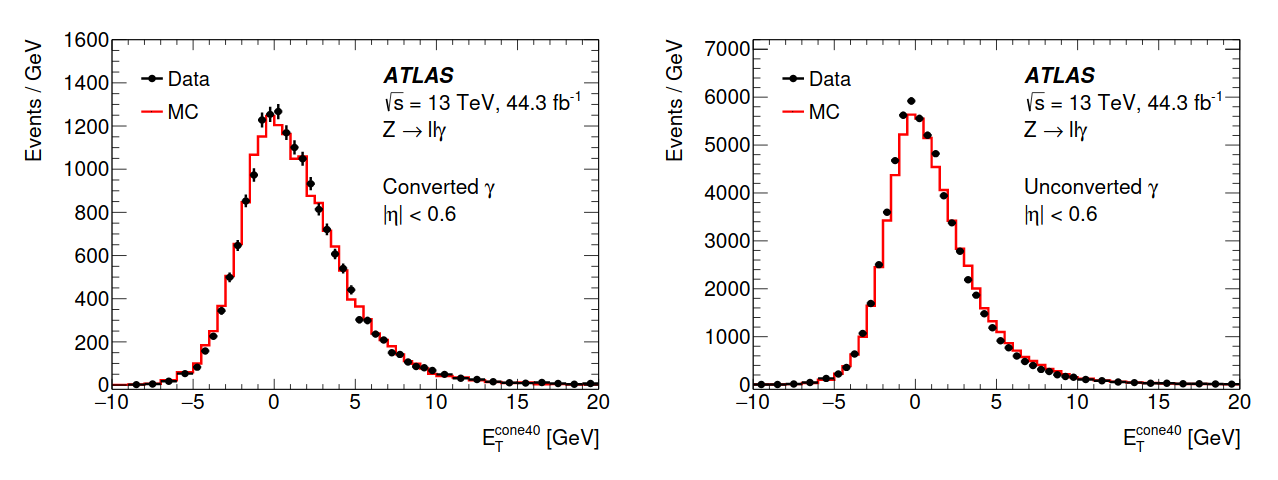
\includegraphics[width=0.85\textwidth]{Ch3/Img/photon_shifts_iso.png}
    \caption{Distribution of $E^{cone40}_T$ in data and simulation, in the central region of the detector ($|\eta|<$0.6), separately for converted (left) and unconverted (right) photons after the data-driven shifts are applied.}
    \label{fig:gamma:Iso:Shifts}
\end{figure}
Figure \ref{fig:gamma:Iso:Eff} shows the efficiency of the isolation WPs defined in Table \ref{tab:gamma:Iso:WPs}, using $Z\rightarrow ll\gamma$ ($l=e, \mu$). The radiative Z decays signature is used to estimate the photon efficiencies as it provides a clean environment of prompt photons, especially in the low-\eT range. 
\begin{figure}[htbp]
    \centering
    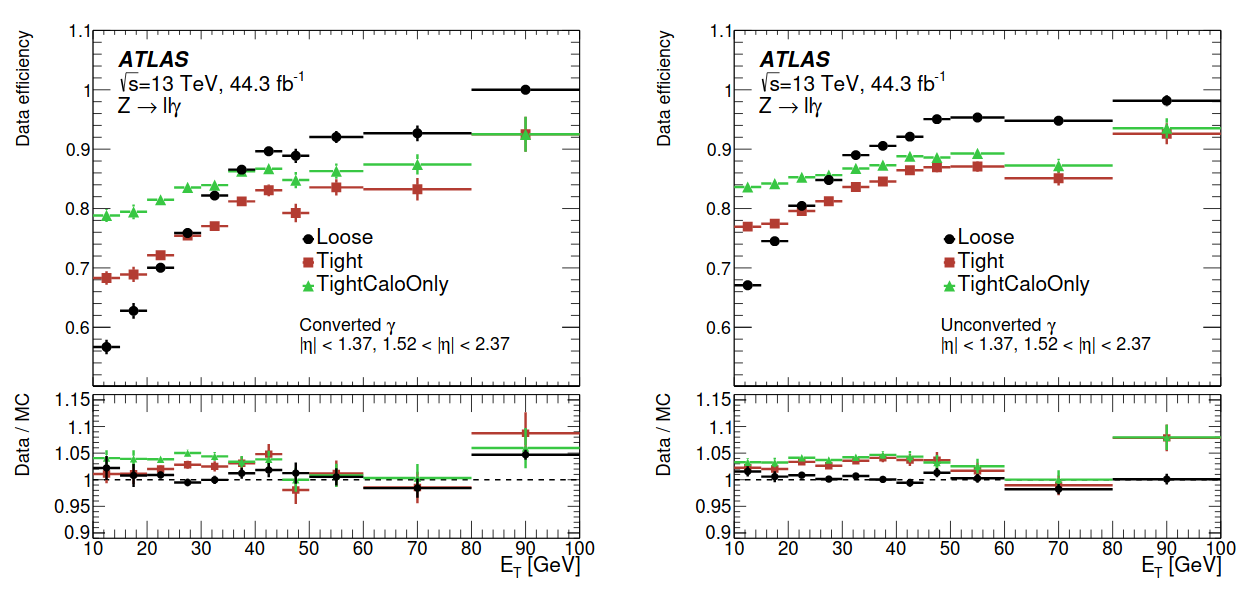
\includegraphics[width=0.85\textwidth]{Ch3/Img/Photon_Iso_Eff.png}
    \caption{Efficiency of the isolation working points for converted(left) and unconverted (right) photons as a function of photon \eT. The lower panel shows the ratio of the efficiencies measured in data and in simulation (scale factors). TThe error bars account for the systematic and statistical errors.}
    \label{fig:gamma:Iso:Eff}
\end{figure}

\section{Photon Identification}
\label{gamma:ID}
In contrary to electron identification, photon identification still relies on rectangular selection criteria, \textit{cut-based algorithm}, using a set of global variables which characterize the lateral and longitudinal electromagnetic shower development in the calorimeter and encode separation between prompt-photons and background photons: non-prompt originating from the decay of QCD jets, and objects misidentification as photons. Such variables, listed in Table \ref{tab:chap2:Objects:Egamma:SS} and depicted in Figure \ref{fig:gamma:ID:SS} with their respective definitions, are called "shower shapes". Given the fine granularity of the first EM layer, the associated shower shapes play an important role to reject the collimated photons from $\pi^{0} \rightarrow\gamma\gamma$ decay. \\ 
\begin{figure}[htbp]
    \centering
    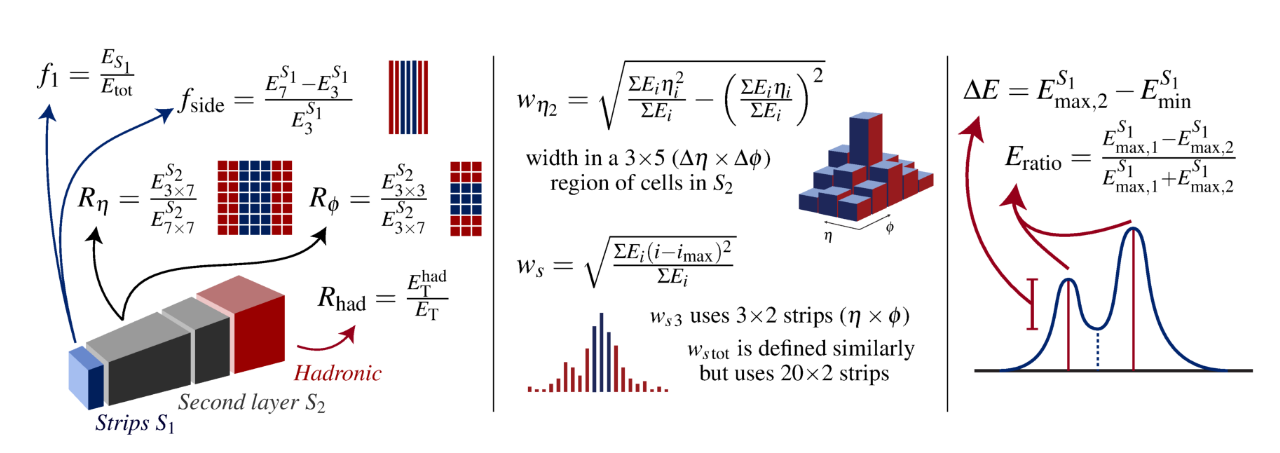
\includegraphics[width=0.85\textwidth]{Ch3/Img/ShowerShapes.png}
    \caption{Schematic representation of the photon identification discriminating variable \cite{ShowerShapes_fig}.}
    \label{fig:gamma:ID:SS}
\end{figure}
\\
The cut-based algorithm provides three WPs: \texttt{Tight}, \texttt{Medium} and \texttt{Loose}, with less restrictive selections respectively. \texttt{Medium} and \texttt{Loose} WPs are mainly used for trigger purposes. Since the trigger system is transparent between converted and unconverted photons, they are similar for both converted and unconverted. Table \ref{tab:gamma:ID:Var} lists the variables set used in each WP. The optimization of the WPs is done using TMVA \cite{TMVA} in bins of $|\eta|$ since the shower shapes vary due to calorimeter granularity. Since the shower shapes are different between the converted and unconverted photons due to the opening angle of the $e^+e^-$ conversion pair and the material interaction, the optimization of tight WP is performed separately for converted and unconverted photons. The tight WP comes with two versions: \eT-independent selection and the \eT-dependent which is tuned in separate bins of $E_T$. The tuning is done in two energy regimes with two different series of the simulated dataset. For photons with 10 $<$ \eT $<$ 25 GeV, the $Z\rightarrow ll\gamma$ simulated sample is used to define the signal, while the corresponding background is derived from the $Z\rightarrow ll+jets$ simulated sample. For \eT $>$ 25 GeV, the inclusive-photon production simulated sample is used as a signal, and the background is the dijet sample. The simulated samples are described in Section 3.1 and 3.2 of Ref. \cite{Egamma_Perf_2017}.   
\begin{table}[htbp]
    \centering
    \begin{tabular}{lc}
        \hline\hline
        Working Point & Variables set \\
        \hline
        \texttt{Loose} & \Rhad, \Rhadone, \Reta \ and \wetatwo \\ 
        \texttt{Medium} & \texttt{Loose} + \Eratio \\ 
        \texttt{Tight} & \texttt{Medium} + \Rphi, \wthree, \wtot, \Fside, \DeltaE \ and \fI \\ 
        \hline\hline
    \end{tabular}
    \caption{Discriminating variables used for \texttt{Loose}, \texttt{Medium} and \texttt{Tight} photon identification.}
    \label{tab:gamma:ID:Var}
\end{table}
\\
Similarly to the calorimeter based variables for isolation, the shower shapes variables suffer from the mis-modelling. The mis-modelling is addressed by setting a data-driven correction similar to the one applied for isolation variables. Corrections are applied as a simple shift to simulated events to align with the real data distributions. Shifts are derived using a $\chi^2$ minimization between the data and simulation in bins of $|\eta|$ and \eT as described in Ref \cite{Photon_Eff_2015}. Figure \ref{fig:gamma:ID:SS:Corr} shows examples of shower shape distributions before and after correction compared to the real distributions using radiative Z photons. Section \ref{gamma:ss} is dedicated to the shower shape mis-modelling and its correction using an alternative method.
\begin{figure}[htbp]
    \centering
    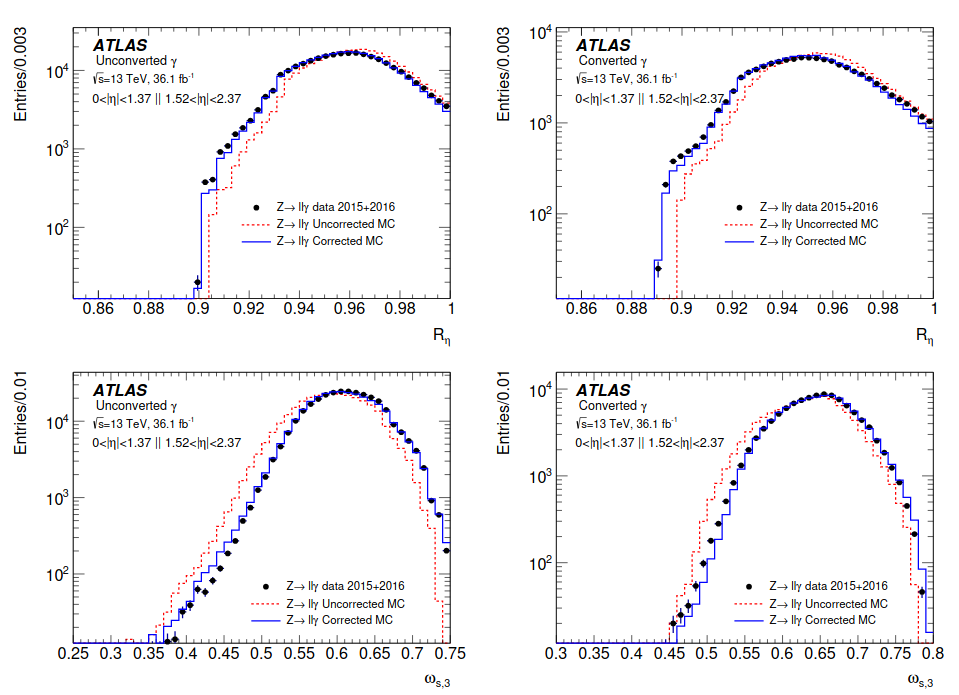
\includegraphics[width=0.75\textwidth]{Ch3/Img/SS_correction.png}
    \caption{Distributions of the \Reta and \wthree \ for converted and unconverted photon candidates with \eT in [10, 50] GeV and $|\eta| < $ 2.37 selected from radiative Z events for data (black), uncorrected simulation (dashed red line) and corrected simulation (solid blue line).}
    \label{fig:gamma:ID:SS:Corr}
\end{figure}
\\
Photon identification efficiency is measured using three different methods over distinct energy regimes:
\begin{itemize}
\item The Matrix Method (MM): based on the inclusive-photon production sample collected using single-photon triggers and performed over a wide kinematic range from 25 GeV to 1.5 TeV in \eT. 
\item The Radiative Z method: uses the clean signature of radiative Z at low-energy and allows a measurement of identification efficiency $\epsilon_{ID}$ from \eT = 10 GeV to 100 GeV. This method handles small background contamination from Z+jets where the jet is misidentified as a photon using a maximum-likelihood fit \cite{Photon_Eff_Run1}. 
\item Electron Extrapolation (EE): uses a transformed electron shower shapes sample form $Z\rightarrow e^+e^-$ and measures $\epsilon_{ID}$ in the region 25 $<$ \eT $<$ 150 GeV.
\end{itemize}
These methods are fully described in Section 5 of Ref. \cite{Photon_Eff_2015}. The tight identification efficiencies from each method are then combined to provide a $\epsilon_{ID}$ measurement for the \eT-dependent selection as shown in Figures \ref{fig:gamma:ID:Eff:UnCov} and \ref{fig:gamma:ID:Eff:Cov}. 
\begin{figure}[htbp]
    \centering
    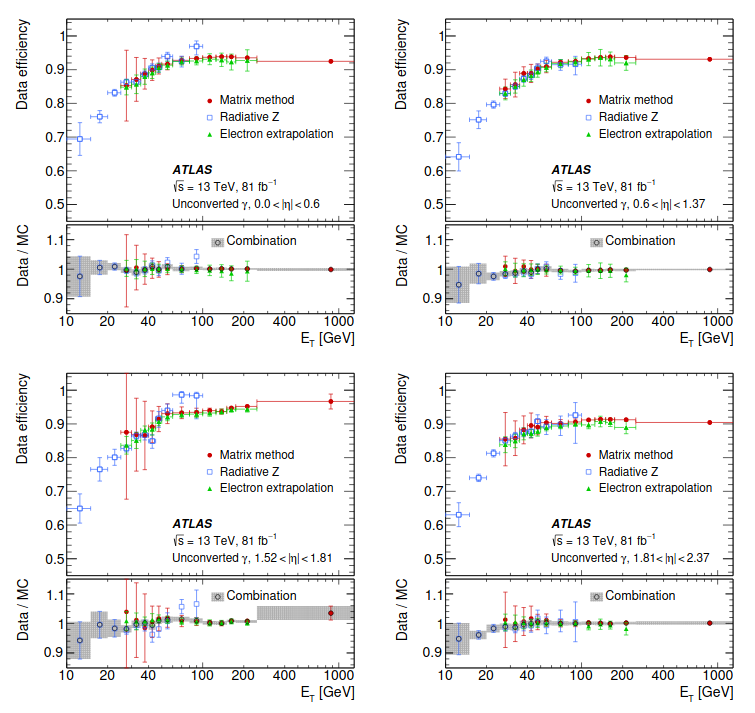
\includegraphics[width=0.6\textwidth]{Ch3/Img/Unconverted_Eff_2017.png}
    \caption{The photon identification efficiency with \eT-dependent selection, and the ratio of data to simulation efficiencies, for unconverted photons with a Loose isolation requirement applied as pre-selection, as a function of \eT in four different $|\eta|$ regions. The combined scale factor, obtained using a weighted average of scale factors from the individual measurements, is also presented; the band represents the total uncertainty.}
    \label{fig:gamma:ID:Eff:UnCov}
\end{figure}
\begin{figure}[htbp]
    \centering
    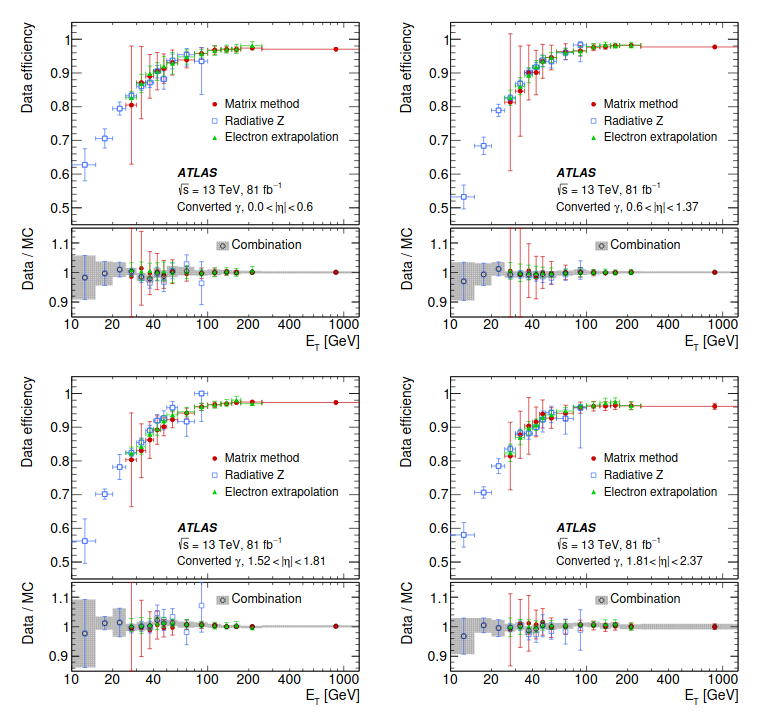
\includegraphics[width=0.6\textwidth]{Ch3/Img/Converted_Eff_2017.png}
    \caption{The photon identification efficiency with \eT-dependent selection, and the ratio of data to simulation efficiencies, for converted photons with a Loose isolation requirement applied as pre-selection, as a function of \eT in four different $|\eta|$ regions. The combined scale factor, obtained using a weighted average of scale factors from the individual measurements, is also presented; the band represents the total uncertainty.}
    \label{fig:gamma:ID:Eff:Cov}
\end{figure}
A comparison between the two versions of the tight WP is shown in Figure \ref{fig:gamma:ID:Eff:Tight}.
\begin{figure}[htbp]
    \centering
    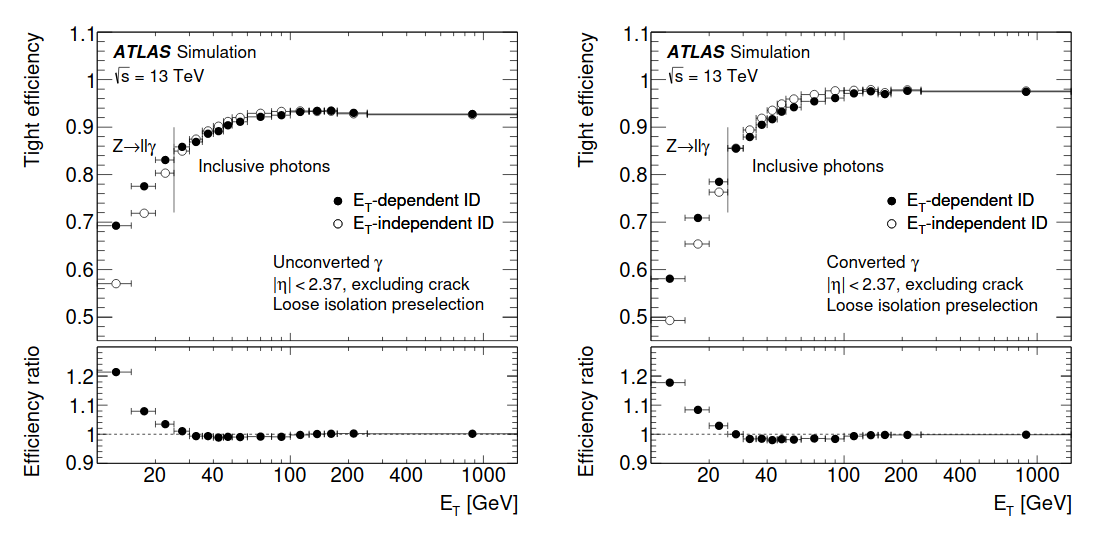
\includegraphics[width=0.75\textwidth]{Ch3/Img/Tight_ID.png}
    \caption{Efficiencies of the tight photon identification for unconverted (left) and converted (right) signal photons, plotted as a function of photon \eT. The loose isolation is applied as a pre-selection. For both plots, the bottom panel shows the ratios between the \eT-dependent and the \eT-independent identification efficiencies.}
    \label{fig:gamma:ID:Eff:Tight}
\end{figure}

\section{Shower shape mis-modelling}
\label{gamma:ss}
The source of the disagreement in shower shapes between the data and the Monte Carlo simulation (MC) described above is still unclear. Many sources can contribute to this mis-modelling, mainly from the detector geometry, material distribution and EM shower modelling. It is difficult to handle those sources and fix the mis-modelling. To fix the issue for electron, a cell-based reweighting method has been developed to apply a global correction to reduce systematic uncertainties related to the mis-modelling \cite{xu, khandoga}. The approach shows a promising electron result, which motivated its application to photons. This work was done in the context of my ATLAS qualification task to allow me to sign ATLAS publications.

\subsection{Cell-based reweighting correction}
\label{gamma:ss:reweighting}
The aim is to redistribute the energy between the cluster cells in simulation to become consistent with the real data. The cell-based reweighting is derived for the second layer of the EM calorimeter. A cluster of 7$\times$11 (7 cells in $\eta$ and 11 cells in $\phi$) centred around the cell with the highest energy (hottest) is considered. The correction is derived as a matrix (7$\times$11) in bins of $\eta$ in two steps:
\begin{enumerate}
    \item Compute single cell corrections as: 
    \begin{equation}
        M_{i}^{\text{Correction}} = \frac{E_{i}^{\text{data}}}{\sum E_{i}^{\text{data}}} -  \frac{E_{i}^{\text{simulated}}}{\sum E_{i}^{\text{simulated}}},
    \end{equation}
    where $E_{i = 1 .. 77}$ denotes the cell energy in the 7$\times$11 cluster of layer 2. 
    \item Compute the reweighted energy for each cluster cell as: 
    \begin{equation}
        E_{i}^{\text{reweighted}} = E_{i}^{\text{non-reweighted}}(1+M_{i}^{\text{Correction}}).
    \end{equation}
\end{enumerate}
The main idea behind the reweighting is to factorize out the material effects and not the physics behaviours, especially the bremsstrahlung tails in the energy profile for electrons and positrons. For electron only, the bremsstrahlung tails are extracted from the $e^+$ and $e^-$ energy profiles as: 
\begin{equation}
E_{i}=\left\{\begin{array}{l}
E_{i}^{\text {electron }} \text { if } E_{i}^{\text {electron }}<E_{i}^{\text {positron }} \\
E_{i}^{\text {positron }} \quad \text { otherwise }
\end{array}\right.
\end{equation}
so it is derived independently of bremsstrahlung and similarly for both electrons and positrons.

\subsection{Electron results}
Figure \ref{fig:gamma:ss:reweighting:electron} shows a reduction in data-simulation discrepancy after the reweighting and leads to a similar distribution for shower shapes computed from layer 2 ($R_{\eta}$ and $R_{\phi}$) between data and simulation.
\begin{figure}[htbp]
    \centering
    \subfloat[][]{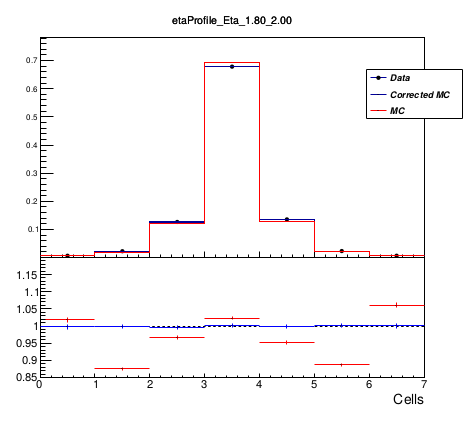
\includegraphics[width=.35\textwidth]{Ch3/Img/etaProfile_Reweighted_Zee.png}}
    \subfloat[][]{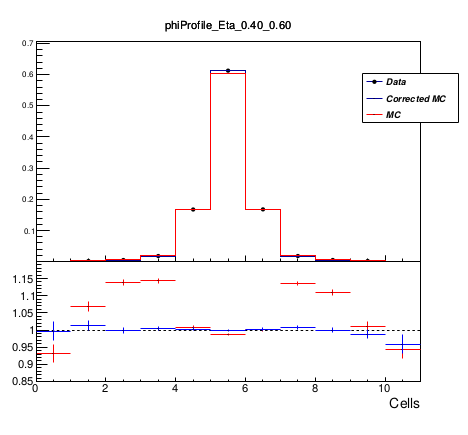
\includegraphics[width=.35\textwidth]{Ch3/Img/phiProfile_Reweighted_Zee.png}} \\
	\subfloat[][]{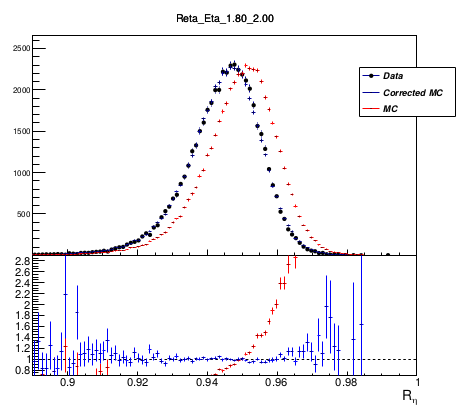
\includegraphics[width=.35\textwidth]{Ch3/Img/Reta_Reweighted_Zee.png}}
	\subfloat[][]{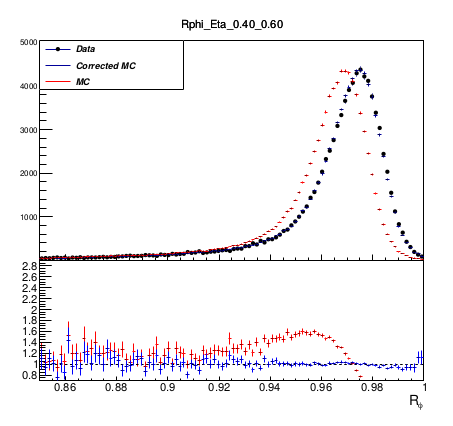
\includegraphics[width=.35\textwidth]{Ch3/Img/Rphi_Reweighted_Zee.png}}
    \caption{(a) Energy profile in $\eta$ direction, (b) Energy profile in $\phi$ direction, (c) $R_{\eta}$ variable and (d) $R_{\phi}$ variable before (red) and after reweighting for electrons from $Z\rightarrow e^+e^-$ for 1.80 $ < |\eta| < $ 2.00 first column and 0.40 $ < |\eta| < $ 0.60 in the second column (the bottom plot is the data/simulation ratio) \cite{khandoga}.}
    \label{fig:gamma:ss:reweighting:electron}
\end{figure}
The cell-based reweighting seems to be promising to reduce data-simulation mis-modelling on electrons shower shapes. Applying the same strategy to photons is the aim of this study. 

\subsection{Cell-based reweighting for photons}
\label{gamma:ss:reweighting:photon}

\subsubsection{Event selection}
\label{gamma:ss:reweighting:photon:RadZSel}
For this study, inclusive photons from $Z\rightarrow ll\gamma$ events are considered. The \verb|SHERPA| generator is used for simulated samples while the data correspond to the 2017 proton-proton collisions. The selection criteria applied are the following:
\begin{enumerate}
    \item Photon selection:  
    \begin{itemize}
    \item Transverse energy \eT $> $  10 GeV.
    \item Pseudorapidity $|\eta|$ within the calorimeter acceptance: $|\eta| < $ 2.37, excluding the transition region between the barrel and end-cap (crack region): 1.37 $ < |\eta| < $ 1.52
    \item Isolation: tight.
    \item Identification: None. 
\end{itemize}
    \item Electron selection:
    \begin{itemize}
        \item Transverse energy \eT $> $  10 GeV.
        \item Pseudorapidity $|\eta| < $ 1.37 or $1.52 < |\eta| < $ 2.47.
        \item Longitudinal impact parameter $z_0 < $ 10 mm, transverse impact parameter significance $|d_0|/\sigma_{d_0}$ less than 10.
        \item Isolation: loose.
        \item Identification: medium.
    \end{itemize}
    \item Combined muon selection: 
    \begin{itemize}
        \item Transverse energy \eT $> $  10 GeV.
        \item Pseudorapidity $|\eta| < $ 2.5.
        \item Longitudinal impact parameter $z_0 < $ 10 mm, transverse impact parameter significance $|d_0|/\sigma_{d_0}$ less than 10.
        \item Isolation: loose.
        \item Identification: medium.
    \end{itemize}
    \item $Z \rightarrow ll\gamma$ event selection:
    \begin{itemize}
        \item $\Delta R_{min}(e,\gamma) > $ 0.4 and $\Delta R_{min}(\mu,\gamma) > $ 0.2: the selection is tighter for electron channel to reduce photon from electron bremsstrahlung.
        \item 80 $ < m_{ll\gamma} < $ 100 GeV to select Z peak,  and 40 $ < m_{ll} < $ 83 GeV for final state radiation (FSR) event selection. 
    \end{itemize}
\end{enumerate}
No identification criteria is applied to photons to avoid any bias from the identification.

\subsubsection{Electrons reweighting applied to photons}
The first strategy has been to apply the electron reweighting values to photons. The developed reweighting matrix for electrons is directly applied to the selected photons from radiative Z events. Figure \ref{fig:gamma:ss:reweighting:photon:electron} shows the energy profiles and layer-2 shower shapes variables before and after the reweighting. The reweighting goes in the correct direction but not enough to correct photons shower shape mis-modelling; this motivates to implement a specific reweighting for photons. Additional control plots for other $\eta$ regions and converted photons are provided in Appendix \ref{Adx1:Electron}.
\begin{figure}[htbp]
    \centering
	\subfloat[][]{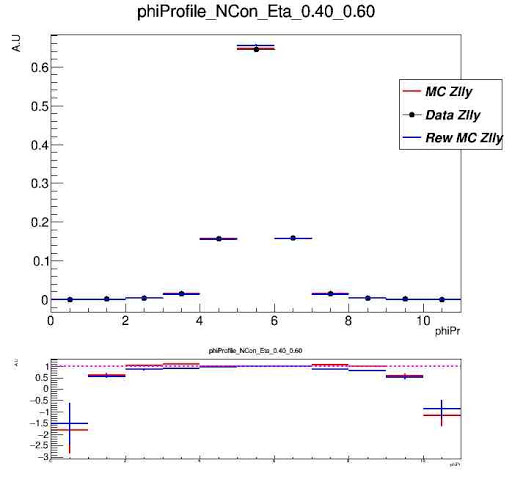
\includegraphics[width=.35\textwidth]{Ch3/Img/phiProfile_NCon_Eta_0.40_0.60.jpg}}
	%\subfloat[][]{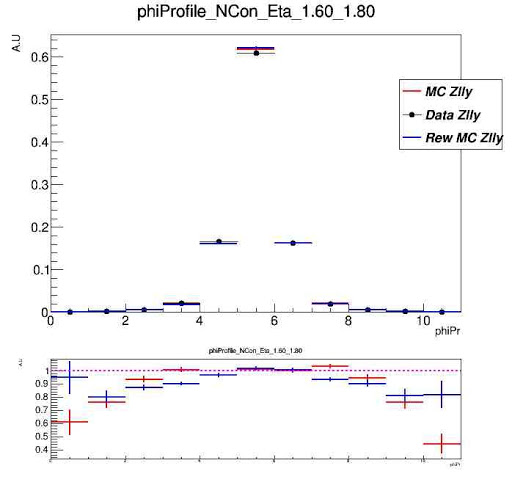
\includegraphics[width=.25\textwidth]{Ch3/Img/phiProfile_NCon_Eta_1.60_1.80.jpg}} 
	%\subfloat[][]{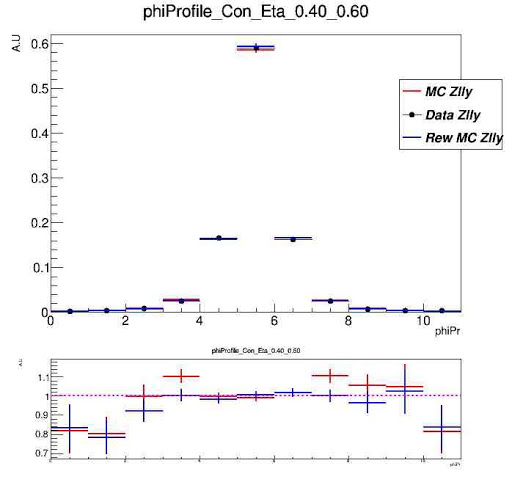
\includegraphics[width=.25\textwidth]{Ch3/Img/phiProfile_Con_Eta_0.40_0.60.jpg}}
	%\subfloat[][]{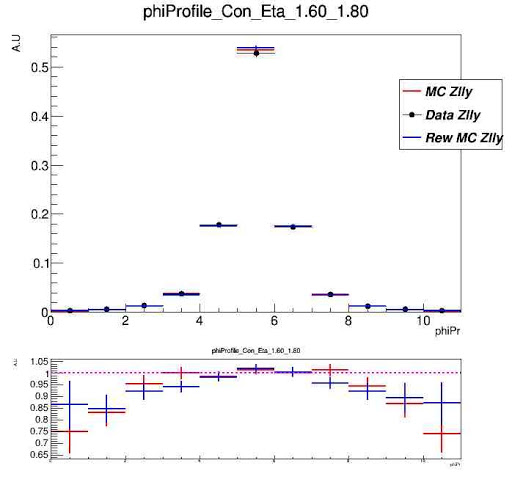
\includegraphics[width=.25\textwidth]{Ch3/Img/phiProfile_Con_Eta_1.60_1.80.jpg}} \\
	\subfloat[][]{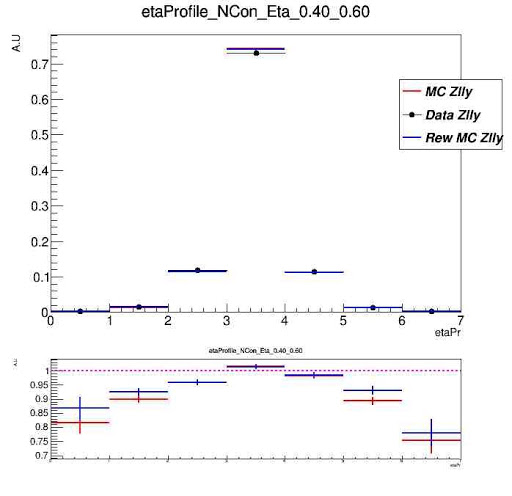
\includegraphics[width=.35\textwidth]{Ch3/Img/etaProfile_NCon_Eta_0.40_0.60.jpg}} \\
	%\subfloat[][]{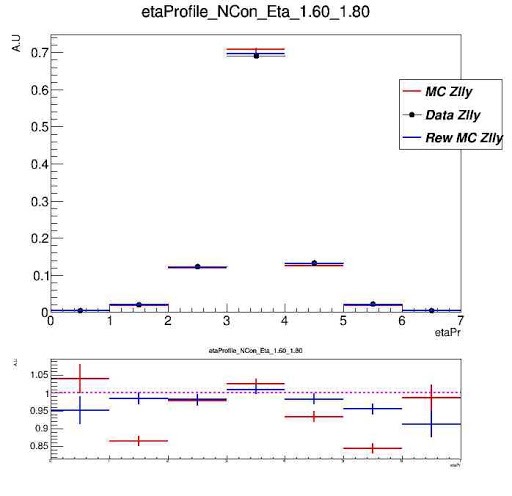
\includegraphics[width=.25\textwidth]{Ch3/Img/etaProfile_NCon_Eta_1.60_1.80.jpg}} 
	%\subfloat[][]{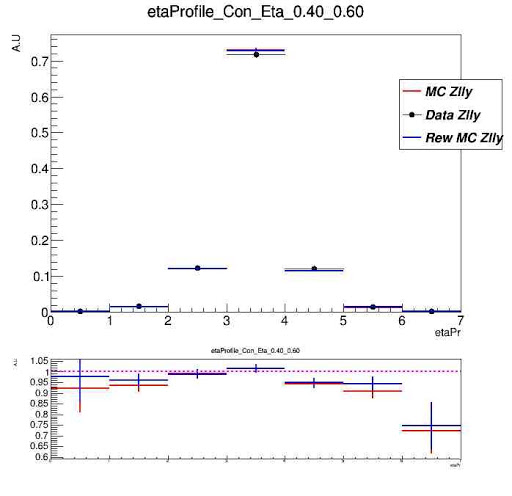
\includegraphics[width=.25\textwidth]{Ch3/Img/etaProfile_Con_Eta_0.40_0.60.jpg}}
	%\subfloat[][]{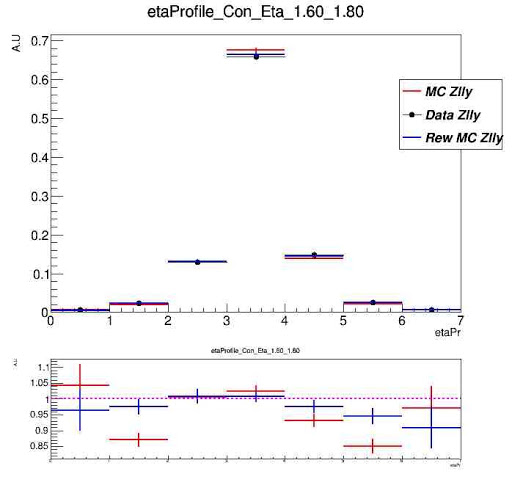
\includegraphics[width=.25\textwidth]{Ch3/Img/etaProfile_Con_Eta_1.60_1.80.jpg}} \\
	\subfloat[][]{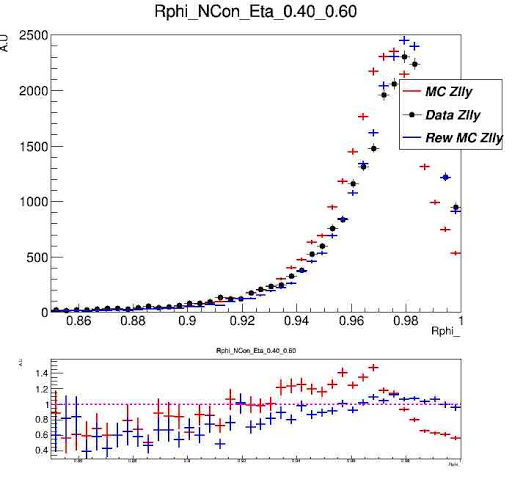
\includegraphics[width=.35\textwidth]{Ch3/Img/Rphi_NCon_Eta_0.40_0.6.jpg.jpg}}
	%\subfloat[][]{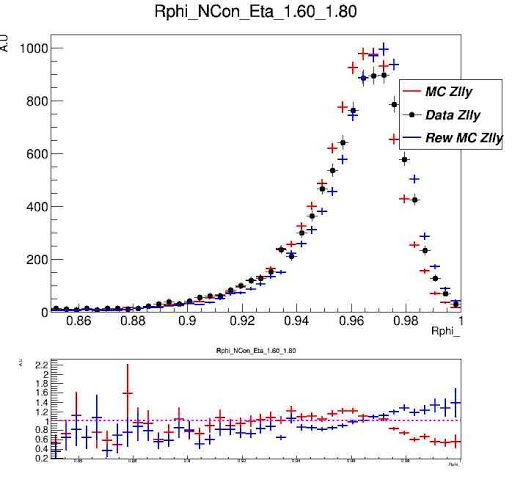
\includegraphics[width=.25\textwidth]{Ch3/Img/Rphi_NCon_Eta_1.60_1.80.jpg}}
	%\subfloat[][]{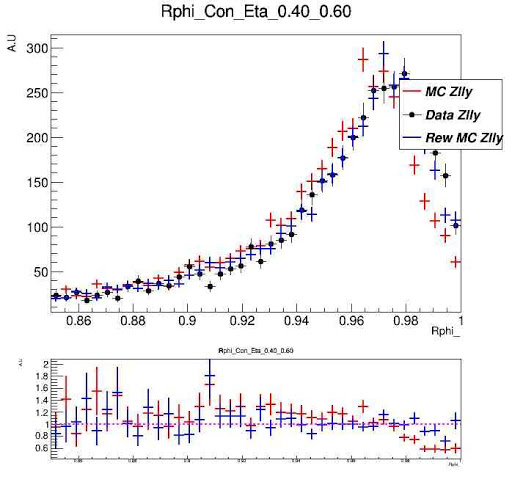
\includegraphics[width=.25\textwidth]{Ch3/Img/Rphi_Con_Eta_0.40_0.6.jpg}}
	%\subfloat[][]{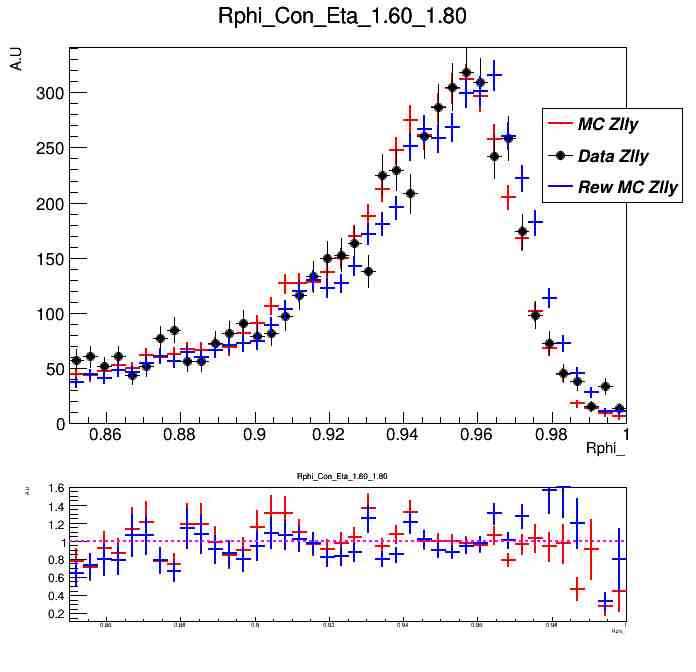
\includegraphics[width=.25\textwidth]{Ch3/Img/Rphi_Con_Eta_1.60_1.80.jpg}} \\
	\subfloat[][]{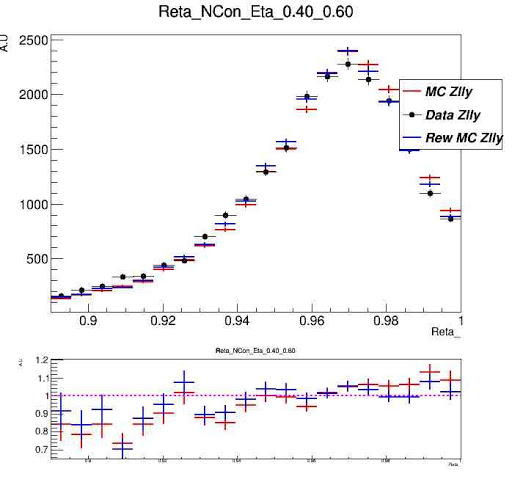
\includegraphics[width=.35\textwidth]{Ch3/Img/Reta_NCon_Eta_0.40_0.6.jpg.jpg}}
	%\subfloat[][]{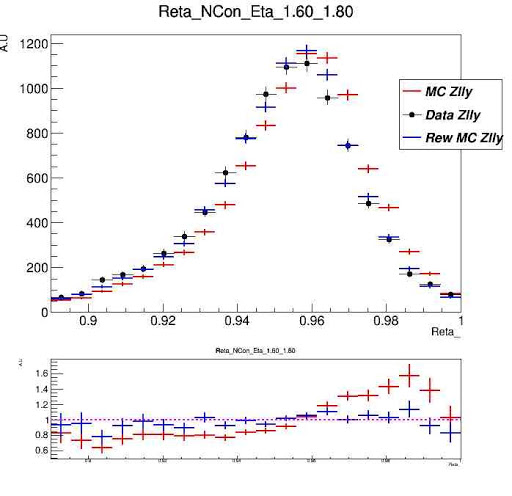
\includegraphics[width=.25\textwidth]{Ch3/Img/Reta_NCon_Eta_1.60_1.80.jpg}}
	%\subfloat[][]{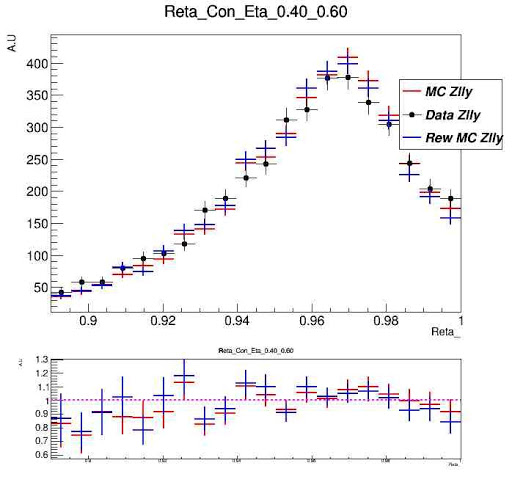
\includegraphics[width=.25\textwidth]{Ch3/Img/Reta_Con_Eta_0.40_0.6.jpg}}
	%\subfloat[][]{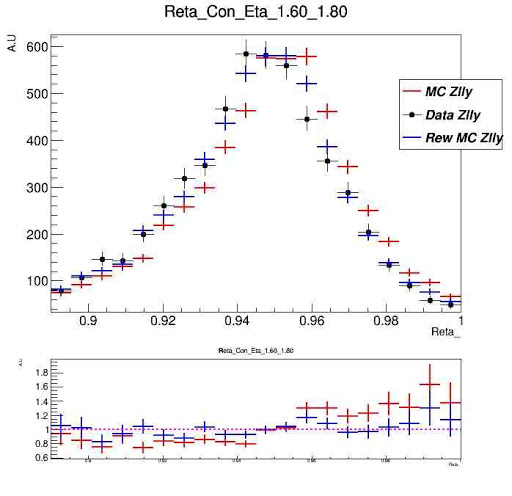
\includegraphics[width=.25\textwidth]{Ch3/Img/Reta_Con_Eta_1.60_1.80.jpg}}
	\begin{tcolorbox}[colback=black!5!white,colframe=white!75!black]
    \caption{The energy profile in $\phi$ and $\eta$ directions (a, b) and the corresponding \Rphi and \Reta variables, for unconverted photons with 0.40 $ < |\eta| < $ 0.60. The black points correspond to Data 2017, red points to non-reweighted simulation and blue points to the reweighted simulation from $Z\rightarrow ll\gamma$.}
    \label{fig:gamma:ss:reweighting:photon:electron}
    \end{tcolorbox}
\end{figure}

\subsubsection{Photon reweighting}
The second step was to derive specific reweighting values for photons. Similarly to electrons, the reweighting is recomputed for photons using radiative Z events inclusively in conversion to reduce statistical uncertainties. Figure \ref{fig:gamma:ss:reweighting:photon:photon} shows the profiles and shower shapes after applying the derived reweighting on photons. A good agreement is observed in energy profiles for both direction $\eta$ and $\phi$. However, for shower shape variables, no significant improvement is observed and the reweighting method seems not to be working for photons. From the energy profiles in Figures \ref{fig:gamma:ss:reweighting:photon:electron} and \ref{fig:gamma:ss:reweighting:photon:photon} photons reweighting from radiative Z are larger than the one for electrons. Additional control plots for other $\eta$ regions and converted photons are provided in Appendix \ref{Adx1:Photon}. To validate the reweighting procedure a closure test is performed on pseudo data (PS).
\begin{figure}[htbp]
    \centering
	\subfloat[][]{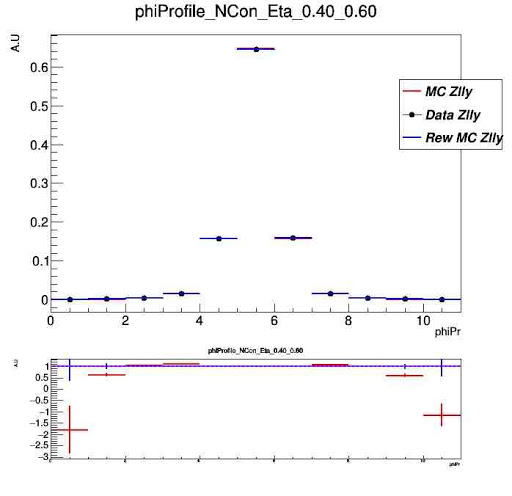
\includegraphics[width=.35\textwidth]{Ch3/Img/PhotonRew/phiProfile_NCon_Eta_0.40_0.60.jpg}}
	%\subfloat[][]{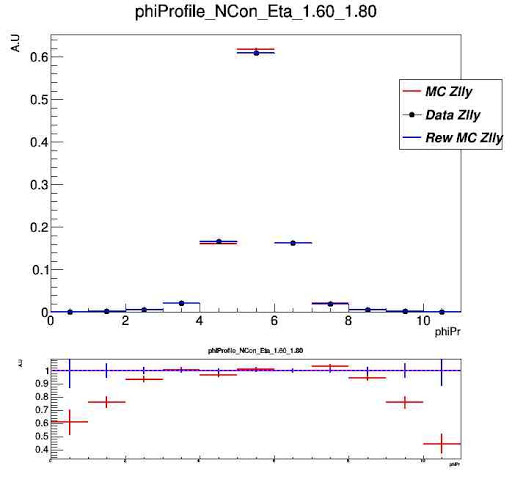
\includegraphics[width=.25\textwidth]{Ch3/Img/PhotonRew/phiProfile_NCon_Eta_1.60_1.80.jpg}} 
	\subfloat[][]{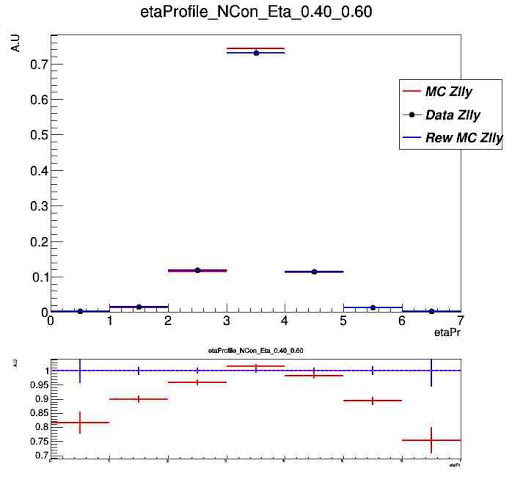
\includegraphics[width=.35\textwidth]{Ch3/Img/PhotonRew/etaProfile_NCon_Eta_0.40_0.60.jpg}} \\
	%\subfloat[][]{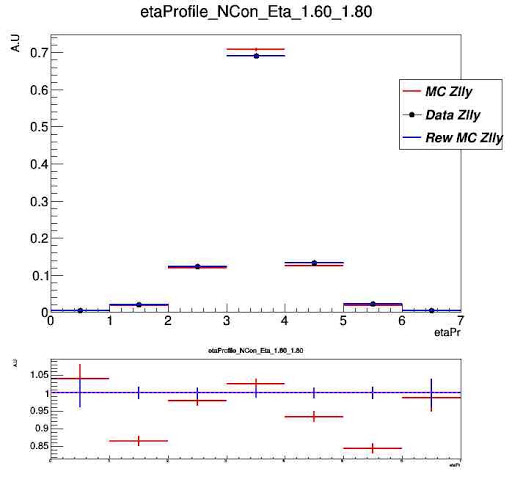
\includegraphics[width=.25\textwidth]{Ch3/Img/PhotonRew/etaProfile_NCon_Eta_1.60_1.80.jpg}} \\
	\subfloat[][]{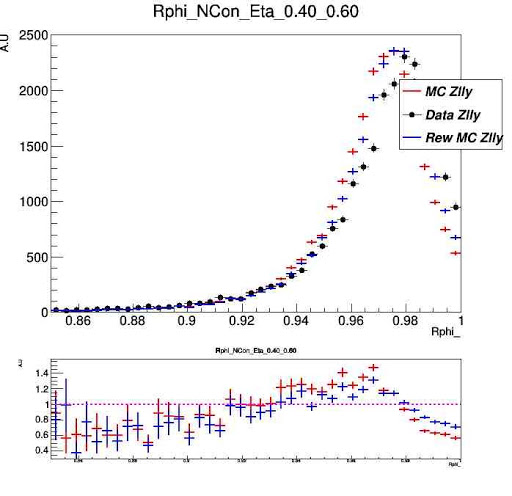
\includegraphics[width=.35\textwidth]{Ch3/Img/PhotonRew/Rphi_NCon_Eta_0.40_0.60.jpg}}
	%\subfloat[][]{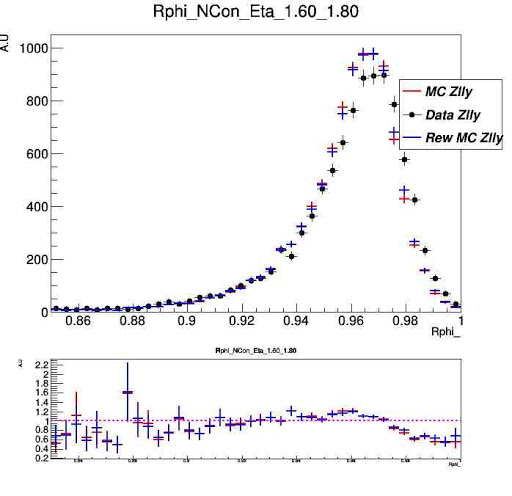
\includegraphics[width=.25\textwidth]{Ch3/Img/PhotonRew/Rphi_NCon_Eta_1.60_1.80.jpg}}
	\subfloat[][]{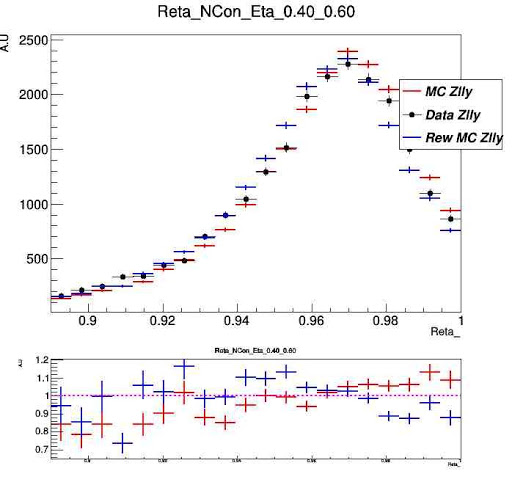
\includegraphics[width=.35\textwidth]{Ch3/Img/PhotonRew/Reta_NCon_Eta_0.40_0.60.jpg}}
	%\subfloat[][]{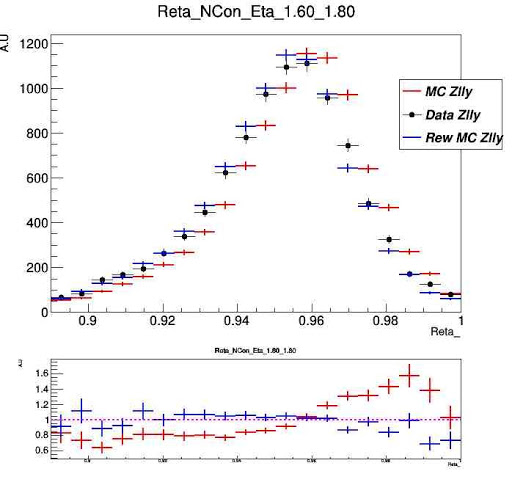
\includegraphics[width=.25\textwidth]{Ch3/Img/PhotonRew/Reta_NCon_Eta_1.60_1.80.jpg}}
	\begin{tcolorbox}[colback=black!5!white,colframe=white!75!black]
    \caption{The energy profile in $\phi$ and $\eta$ directions (a, b) and the corresponding \Rphi and \Reta variables, for unconverted photons with 0.40 $ < |\eta| < $ 0.60. The black points correspond to Data 2017, red points to non-reweighted simulation and blue points to the reweighted simulation from $Z\rightarrow ll\gamma$.}
    \label{fig:gamma:ss:reweighting:photon:photon}
    \end{tcolorbox}
    
\end{figure}

\subsubsection{Closure test}
To validate the implemented code, a closure test was performed using PS from simulation, for that:
\begin{enumerate}
    \item PS is produced by adding 50 MeV (arbitrary value) to each simulated cell.
    \item Re-compute the reweighting function with the same procedure as above using unconverted photons (for simplicity).
    \item Correct simulated cell to match the PS.
\end{enumerate}
Results of the closure test are shown in Figure \ref{fig:gamma:ss:reweighting:photon:closure}. 
\begin{figure}[htbp]
    \centering
	\subfloat[][]{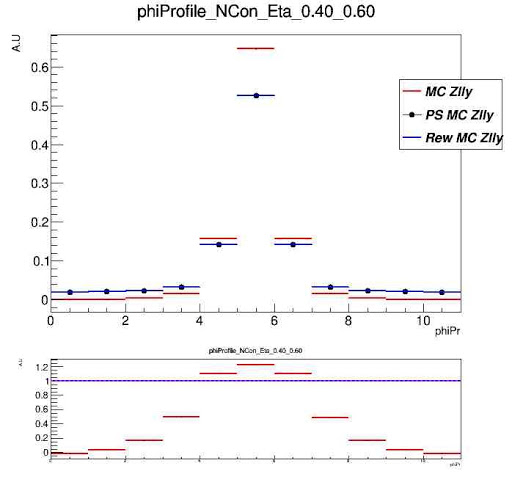
\includegraphics[width=.35\textwidth]{Ch3/Img/PhotonRew/PS_phiProfile_NCon_Eta_0.40_0.60.jpg}}
	%\subfloat[][]{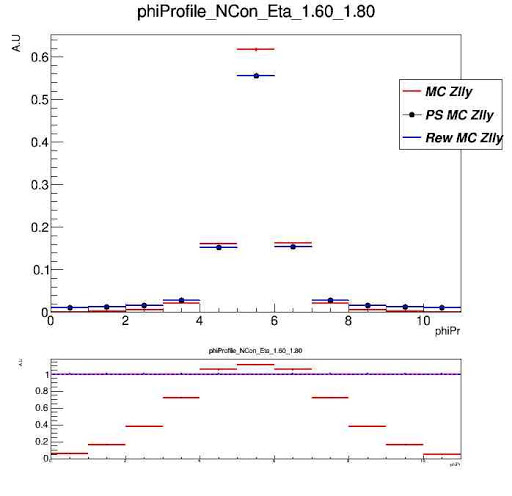
\includegraphics[width=.25\textwidth]{Ch3/Img/PhotonRew/PS_phiProfile_NCon_Eta_1.60_1.80.jpg}}
	\subfloat[][]{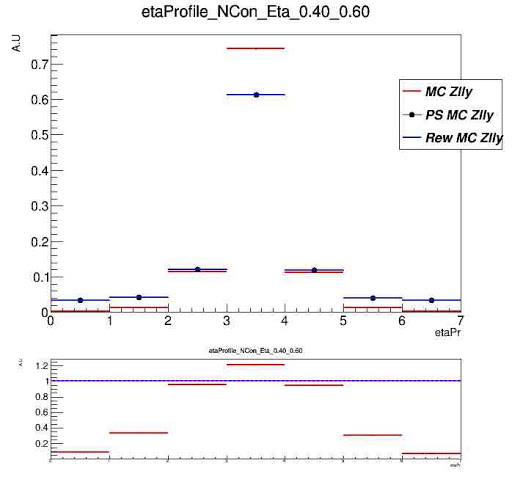
\includegraphics[width=.35\textwidth]{Ch3/Img/PhotonRew/PS_etaProfile_NCon_Eta_0.40_0.60.jpg}} \\
	%\subfloat[][]{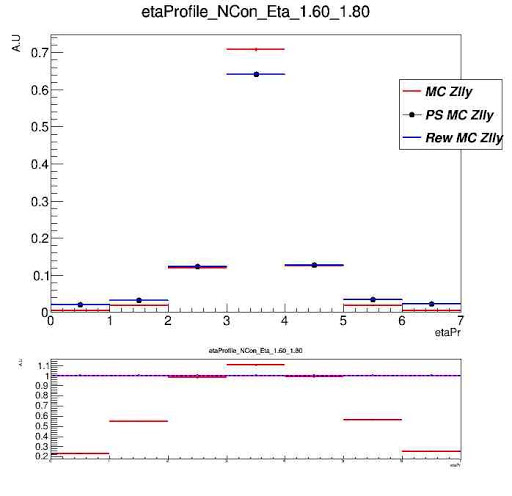
\includegraphics[width=.25\textwidth]{Ch3/Img/PhotonRew/PS_etaProfile_NCon_Eta_1.60_1.80.jpg}} \\
	\subfloat[][]{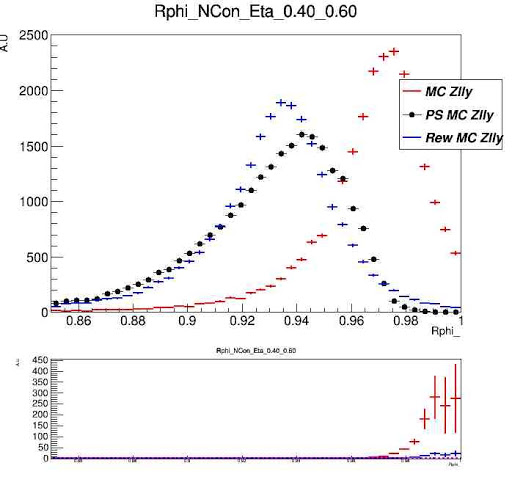
\includegraphics[width=.35\textwidth]{Ch3/Img/PhotonRew/PS_Rphi_NCon_Eta_0.40_0.60.jpg}}
	%\subfloat[][]{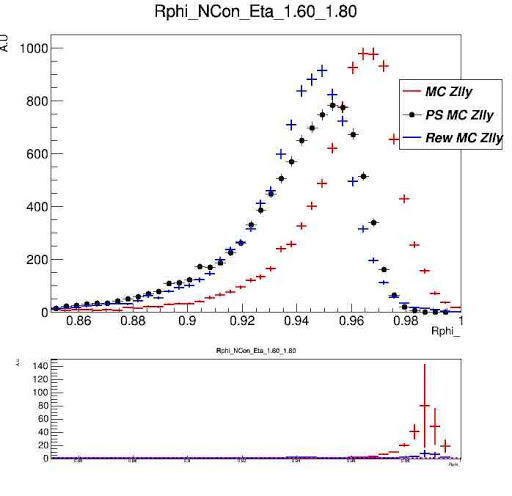
\includegraphics[width=.25\textwidth]{Ch3/Img/PhotonRew/PS_Rphi_NCon_Eta_1.60_1.80.jpg}}
	\subfloat[][]{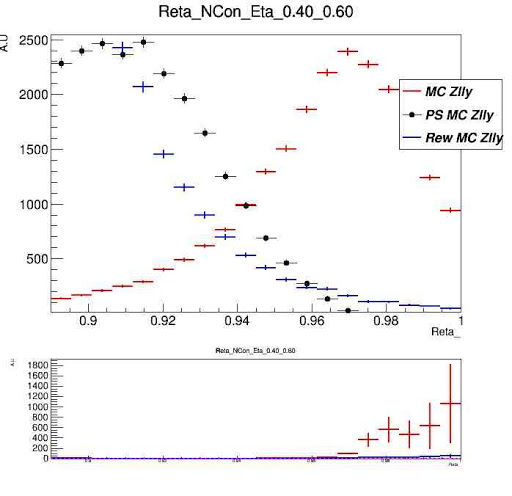
\includegraphics[width=.35\textwidth]{Ch3/Img/PhotonRew/PS_Reta_NCon_Eta_0.40_0.60.jpg}}
	%\subfloat[][]{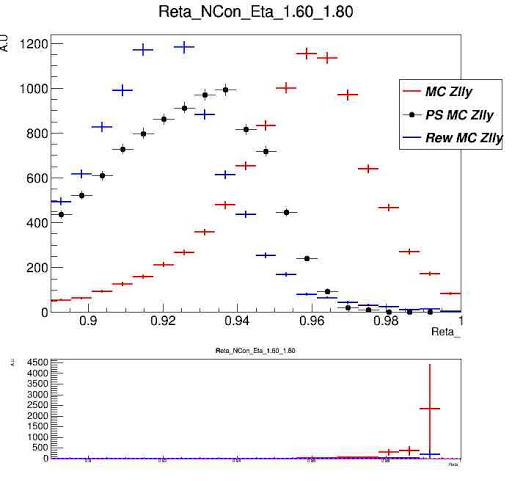
\includegraphics[width=.25\textwidth]{Ch3/Img/PhotonRew/PS_Reta_NCon_Eta_1.60_1.80.jpg}}
	\begin{tcolorbox}[colback=black!5!white,colframe=white!75!black]
    \caption{The energy profile in $\phi$ and $\eta$ directions (a, b) and the corresponding \Rphi and \Reta variables, for unconverted photons with 0.40 $ < |\eta| < $ 0.60. The black points correspond to the pseudo data, red points to non-reweighted simulation and blue points to the reweighted simulation from $Z\rightarrow ll\gamma$.}
    \label{fig:gamma:ss:reweighting:photon:closure}
    \end{tcolorbox}
    
\end{figure}
\\
Perfect agreement in energy profiles for both directions ($\eta$ and $\phi$) is observed. The closure test reproduces the PS, while for shower shapes the agreement is improved in the correct direction but not enough to correct the "fake" mis-modelling. The closure test demonstrates that the reweighting procedure was not able to catch the discrepancy between data and simulation, and seems to be working only on average and not event-by-event. \\
Figure \ref{fig:gamma:ss:reweighting:photon:closure:avg} shows the averages of $R_{\eta}$ and $R_{\phi}$ in real data, simulation and after reweighting in bin of photon $|\eta|$. After reweighting, the average of shower shapes in simulation perfectly matches the data distribution, which demonstrates that the reweighting is working on average and not event-by-event.

\begin{figure}[htbp]
    \centering
    \subfloat[][]{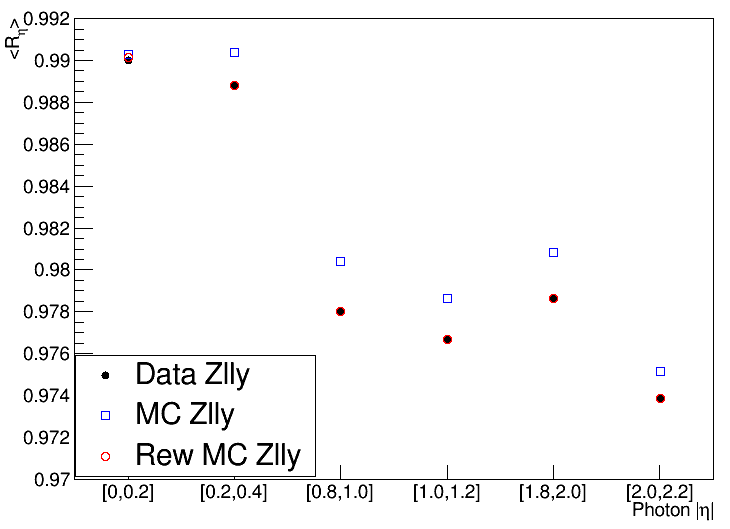
\includegraphics[width=.45\textwidth]{Ch3/Img/PhotonRew/Reta_avg.png}}
    \subfloat[][]{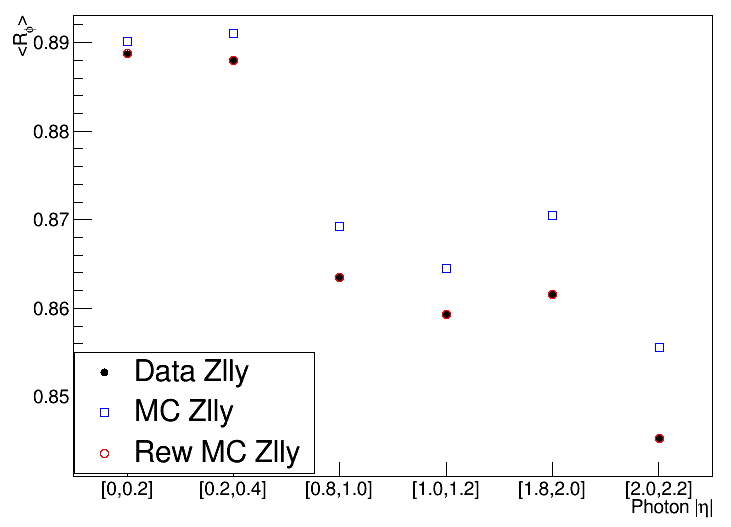
\includegraphics[width=.45\textwidth]{Ch3/Img/PhotonRew/Rphi_avg.png}}
    \begin{tcolorbox}[colback=black!5!white,colframe=white!75!black]
    \caption{Average $R_{\eta}$ (a) and $R_{\phi}$ (b) in real data (black), simulation (blue) and after reweighting (red) using photon reweighting values.}
    \label{fig:gamma:ss:reweighting:photon:closure:avg}
    \end{tcolorbox}
\end{figure}

\label{tab:avg}

%One of the possible reasons why reweighting works for electrons and not for photons is the fact that the reweighting function for electrons benefits from high statistics leads to modulate the energy in each cell with a Gaussian distribution (Central limits theorem) instead of photons which suffer from low statistics and high background contamination. Having more statistics and sophisticated techniques to extract background will helps to generate a reweighting function for photons.

\subsubsection{Three-dimensional reweighting}
Since the reweighting is only correcting on average and not event-by-event, a new reweighting technique was developed which is presented here. The idea is to add cell energy as an additional dimension to the previous reweighting procedure. The reweighting factor for each cell will be a function of cell energy. Instead of 2D reweighting the reweighting will be in three dimensions, defined as:
\begin{equation}
    E_{k,n}^{\text{reweighted}} = E_{k,n}^{\text{non-reweighted}} \times \alpha \ ; \text{with} \ \alpha = f(k,n,E_{k,n}^{\text{simulated}}) = E_{k,n}^{\text{data}}/E_{k,n}^{\text{simulated}},
\end{equation}
where $k$ = 1..77 denotes the cell number, n the corresponding photon $|\eta|$ bin and $E_{k,n}^{\text{simulated}}$  the energy of the cell $k$ in $\eta$ bin n. \\
The new method requires matching between photons from data and simulation to compute the $\alpha$ factors, which is technically complicated. The procedure is tested with PS from simulation. The PS is derived from simulation by scaling the energy of the cell $k$ by 0.26 (the factor 0.26 is arbitrary). For simplicity, the reweighting is evaluated using unconverted photons only.
The result of the new reweighting procedure is presented in Figure \ref{fig:gamma:ss:reweighting:photon:3dreweighting}. A good agreement is observed after the three-dimensional reweighting for both energy profiles and their corresponding shower shapes variables for layer 2. The improvement in data-simulation agreement observed makes the new method promising to be applied on real data.
%This work is kept for the newcomers to the ATLAS collaboration.
\begin{figure}[htbp]
    \centering
	\subfloat[][]{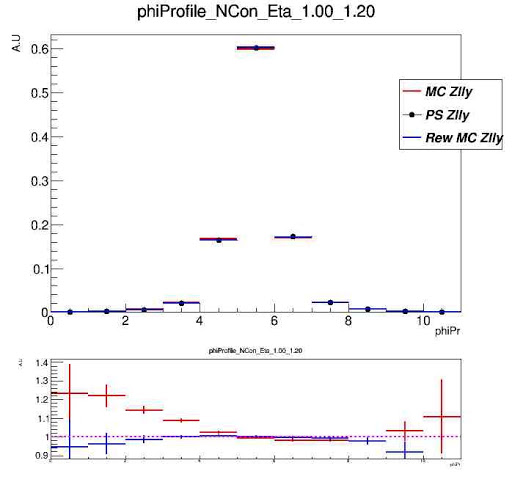
\includegraphics[width=.35\textwidth]{Ch3/Img/PhotonRew/NPS_phiProfile_NCon_Eta_1.0_1.20.jpg}}
	%\subfloat[][]{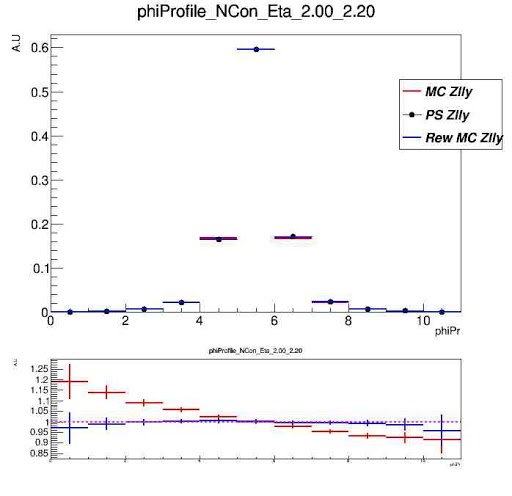
\includegraphics[width=.25\textwidth]{Ch3/Img/PhotonRew/NPS_phiProfile_NCon_Eta_2.20_2.40.jpg}}
	\subfloat[][]{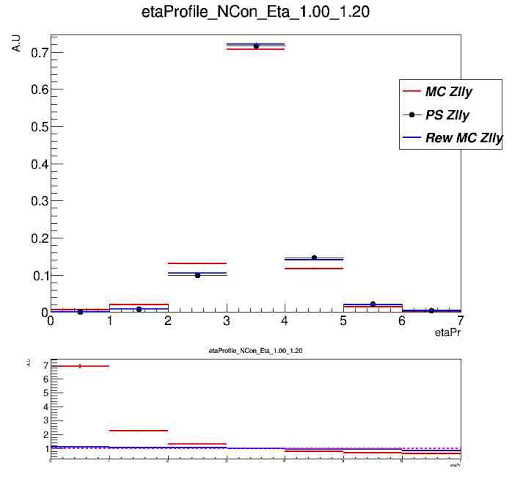
\includegraphics[width=.35\textwidth]{Ch3/Img/PhotonRew/NPS_etaProfile_NCon_Eta_1.0_1.20.jpg}} \\
	%\subfloat[][]{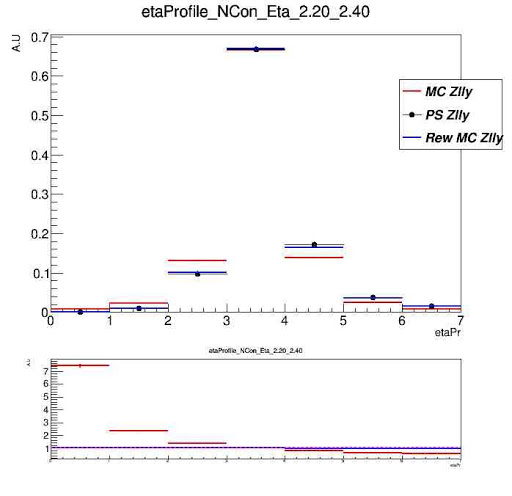
\includegraphics[width=.25\textwidth]{Ch3/Img/PhotonRew/NPS_etaProfile_NCon_Eta_2.20_2.40.jpg}} \\
	\subfloat[][]{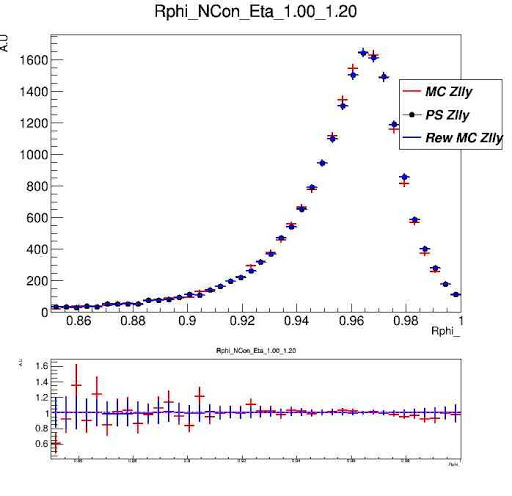
\includegraphics[width=.35\textwidth]{Ch3/Img/PhotonRew/NPS_Rphi_NCon_Eta_1.00_1.20.jpg}}
	%\subfloat[][]{\includegraphics[width=.25\textwidth]{Ch3/Img/PhotonRew/NPS_Rphi_NCon_Eta_2.00_2.20.jpg}}
	\subfloat[][]{\includegraphics[width=.35\textwidth]{Ch3/Img/PhotonRew/NPS_Reta_NCon_Eta_1.00_1.20.jpg}}
	%\subfloat[][]{\includegraphics[width=.25\textwidth]{Ch3/Img/PhotonRew/NPS_Reta_NCon_Eta_2.00_2.20.jpg}}
	\begin{tcolorbox}[colback=black!5!white,colframe=white!75!black]
    \caption{The energy profile in $\phi$ and $\eta$ directions (a, b) and the corresponding \Rphi and \Reta variables, for unconverted photons with 1.00 $ < |\eta| < $ 1.20. The black points correspond to the pseudo data, red points to non-reweighted simulation and blue points to the reweighted simulation from $Z\rightarrow ll\gamma$.}
    \label{fig:gamma:ss:reweighting:photon:3dreweighting}
    \end{tcolorbox}
\end{figure}

\section{Convolutional Neural Network for Photon Identification}
\label{gamma:CNN}
Applying cuts on shower shape variables for the identification algorithm limits the potential to improve the separation between prompt and background photons. Correcting the mis-modelling seems to be a critical problem without any solution for the moment. For these reasons, a further improvement is possible by developing a new identification algorithm based on the EM cells and using advanced Machine Learning (ML) techniques. The EM cells of the photon cluster are commonly represented as an image, where each pixel contains the cell energy, leading to the use of images of the deposited energy in the calorimeter to learn the shower properties. The most adapted ML technique for image processing is Convolutional Neural Networks (CNN). In the following, its implementation using EM calorimeter images is described. A complete description of NNs goes beyond the scope of this thesis. The interested reader can find an introduction to NNs in Ref. \cite{NNs}. 

\subsection{CNN algorithm}
\subsubsection{Event selection}
Simulated samples of inclusive photon production are used to train the CNN. The inclusive photon sample includes $\gamma$+jet events from the hard subprocesses $qg \rightarrow q\gamma$ and $ q\bar{q}\rightarrow g\gamma$ enriched by prompt photon and used as a signal for the training. Background photons are taken from quark fragmentation in QCD di-jet events. Photon candidates are requested to pass the same photon selection defined for radiative Z in Section \ref{gamma:ss:reweighting:photon:RadZSel}. Additionally, photons used as a signal in the training (prompt) are required to be stable particle, not originate from a hadron and to match to a truth photon. Photons failing one of these requirements are flagged as a background. Photons from radiative Z decay are used as a control sample to evaluate the performance of the trained model (out-of-sample validation).

\subsubsection{Images pre-processing}
\label{gamma:CNN:PreProcessing}
To compromise between collecting more energy and minimizing the impact of the activity around the cluster, the 7$\times$11 cluster around the hottest cell is considered similarly to the shower shapes computation. As the EM cell granularity changes with $\eta$ (Table \ref{tab:chap2:ATLAS:Calo:ECal:Gr}), it leads to a different number of cells in each $\eta$ region. The corresponding number of cells in 7$\times$11 windows are summarized in Table \ref{tab:gamma:CNN:PreProcessing:NCells}.
\begin{table}[htbp]
    \centering
    \begin{tabular}{lcccc}
    \hline\hline
        $|\eta|$ range & 0 to 1.4 & 1.4 to 1.8 & 1.8 to 2.0 & 2.0 to 2.5 \\
    \hline
        Sampling 1 & 112 & 112 & 84 & 56 \\
        Sampling 2 & 77 & 77 & 77 & 77 \\
        Sampling 3 & 44 & 44 & 44 & 44 \\
    \hline\hline
    \end{tabular}
    \caption{Number of cells in 7$\times$11 EM calorimeter windows.}
    \label{tab:gamma:CNN:PreProcessing:NCells}
\end{table}
\\
The difference in shape and size of the EM calorimeter windows complicates the network training procedure. To avoid this issue, zeros are appended to the calorimeter cluster image to end up with the same image size in all $\eta$ region for each sampling (e.g., sampling 1 with 84 cells is completed by zeros, to have 112 cells). Table \ref{tab:gamma:CNN:PreProcessing:ImgSize} shows the final image shape used for each sampling.
\begin{table}[htbp]
    \centering
    \begin{tabular}{lc}
    \hline\hline
        Sampling & Shape \\
    \hline
        Sampling 1 & (56, 2)\\
        Sampling 2 & (7, 11)  \\
        Sampling 3 & (4, 11) \\
    \hline\hline
    \end{tabular}
    \caption{Image shape of 7$\times$11 windows in each sampling in ($\eta$, $\phi$).}
    \label{tab:gamma:CNN:PreProcessing:ImgSize}
\end{table}
\\
I decided to use the cell energy normalized to the total cluster energy as an image pixel to build an energy independent algorithm which performs in the same way for all energy regime.

\subsubsection{CNN Architecture}
\label{gamma:CNN:Model}
A CNN classifier is built to separate between prompt and background photons using images of the 7$\times$11 cluster windows of sampling 1, 2, and 3. Figure \ref{fig:gamma:CNN:Model:Idea} shows an illustration of the classifier.
\begin{figure}[htbp]
    \centering
    \includegraphics[width=.5\textwidth]{Ch3/Img/CNN_Idea.png}
    \begin{tcolorbox}[colback=black!5!white,colframe=white!75!black]
    \caption{CNN classifier schema.}
    \label{fig:gamma:CNN:Model:Idea}
    \end{tcolorbox}
\end{figure}
\\
The Global CNN classifier is constructed using the \textsc{Keras} library, with \textsc{Tensorflow} as a backend \cite{keras, tensorflow}. Information from EM layers images is extracted using three baby CNNs. Each one is connected to an EM layer and built from two sets of two-dimensional convolution (2DCov) and two-dimensional max-pooling (2DMaxPool) \cite{maxpooling} layers followed by a flatten layer that prepares a vector for the fully connected network. Output vectors of the three flatten layers are combined using a concatenate layer, then pass through a Dense Neural Network (DNN) for the classification task. The DNN is made of two Dense (fully connected) layers, a dropout, another Dense layer then a final output layer. An illustration of the architecture is given in Figure \ref{fig:gamma:CNN:Model:Arch}. \\
All layers in the network have their weights randomly initialized by sampling from a truncated normal distribution centred on zero with the width given by $\sqrt{1/N_{input}}$, where $N_{input}$ is the number of input units in the weight tensor. The activation function of each layer is Scaled Exponential Linear Unit (SELU) \cite{SELU} to preserve the mean and variance of the inputs between two consecutive layers and handle the normalization issues, except for the final output layer which has "sigmoid" as an activation function.\\
Layers in the babies CNN are 256 nodes wide, while in the DNN 128 nodes except for the output layer is one node wide.\\
Using an output layer with a sigmoid activation function allows interpreting the output as the probability for each class (prompt or background photon), given the input images.\\
\begin{figure}[htbp]
    \centering
    \includegraphics[width=1.\textwidth]{Ch3/Img/CNN_model.png}
    \begin{tcolorbox}[colback=black!5!white,colframe=white!75!black]
    \caption{Illustration of the global CNN classifier graph.}
    \label{fig:gamma:CNN:Model:Arch}
    \end{tcolorbox}
    
\end{figure}
%Dropout layers are a form of statistical learning regularization that is reminiscent of ensemble methods in the non-deep-learning arena, such as random forests \cite{dropout}. They act to randomly disable a tunable fraction (the dropout rate) of inputs at each training step. It prevents nodes within the network from co-adapting too much, thus avoiding/reducing the effects of overtraining/fitting. During each forward pass of a set of inputs through the network, the dropout layers disable portions of the network thereby presenting a modified network to the inputs. After the forward pass of the inputs, the results are then backpropagated also through the same modified network. Conceptually, then, using dropout during training is similar to training a set of very many, different weak neural networks. During test time, the network’s weights, which have been determined after training on the set of thinned networks, are scaled down by the dropout rate. As briefly mentioned above, dropout prevents nodes within the network from co-adapting too much and forces the network to learn more robust features that are useful in conjunction with many different random subsets of the other nodes. That is, dropout ensures that the model is robust against the loss of any individual "piece of evidence" and is found to reduce the effects of overfitting/overtraining thereby increasing the generalizability of the network.
\\
In the network presented, the dropout layer has a dropout rate of 8\%.
During the training, the binary cross-entropy is used as a loss metric, the optimization is done with Adam optimizer.

\subsubsection{CNN Training}
\label{gamma:CNN:Training}
The CNN of $\sim$1.4 million parameters is trained with a learning rate of $1e^{-4}$ and a batch size fixed to 96 images (32 photons) due to memory limitations, with a maximum number of epochs set to 20. CNN network is trained using two NVIDIA Tesla K80 GPUs with a memory of 12 GB each run on CC-In2p3 cluster (France) \cite{cca}. Each training epoch lasts $\sim$15 minutes. An early stopping metric \cite{early} is imposed during the training phase to reduce the over-training/fitting, such that if the network learning reaches the plateau it will stop. The metric used to determine the early stopping is the network loss as evaluated on the validation data sample throughout the training. The network aims to minimize the weighted loss function between the truth and predicted labels.\\
The network is trained inclusively in \eT, $\eta$ and photon conversion type. Only cluster images are included during the training.
Figure \ref{fig:gamma:CNN:Training:loss} shows the evaluation of loss function and the accuracy during the training time for the training and validation dataset. After the 4$^{th}$ epoch the network achieves the plateau and the validation loss does not decrease. To reduce the overtraining, the early stopping metric stops the training at epoch 4.
\begin{figure}[htbp]
    \centering
    \includegraphics[width=.6\textwidth]{Ch3/Img/CNN_Loss_Accuracy.png}
    \begin{tcolorbox}[colback=black!5!white,colframe=white!75!black]
    \caption{Neural network loss and accuracy as function of epoch number.}
    \label{fig:gamma:CNN:Training:loss}
    \end{tcolorbox}
    
\end{figure}

\subsubsection{CNN Validation}
\label{gamma:CNN:Validation}
The CNN output is scanned to compute the improvement in two different approaches in bins of photon $p_T$ and $|\eta|$: 
\begin{itemize}
    \item Background rejection for the same cut-based signal efficiency.
    \item Signal efficiency for the same cut-based background rejection.
\end{itemize} 
The signal efficiency $\epsilon_{eff}$ and background rejection $\epsilon_{rej}$ are evaluated as the following:
\begin{equation}
    \label{eq:eff}
    \epsilon_{eff} = \frac{TP}{TP+FN} \ ; \ \epsilon_{rej} = \frac{TN}{TN+FP},
\end{equation}
where TP is the number of prompt photons correctly classified as a signal by the CNN, TN is the number of background photons correctly classified as background, FP is the number of prompt photons misclassified as background and FN is the number of background photons misclassified as a signal. The following binning is used $p_T$ = [10, 20, 30, 40, 60, 80, $\infty$] GeV and $|\eta|$ = [0., 0.6, 1.37, 1.52, 1.8, 2.4].
Figure \ref{fig:gamma:CNN:Validation:ROC} shows the receiver-operating characteristic (ROC) which illustrates the diagnostic ability of the CNN as its discrimination threshold is varied. The blue dot shows the signal and background rejection of the current cut-based tight WP. A significant improvement is obtained with the CNN compared to tight WP for both converted and unconverted photons. 
\begin{figure}[htbp]
    \centering
   \subfloat[][]{\includegraphics[width=.5\textwidth]{Ch3/Img/ROC_UnConverted.png}}
	\subfloat[][]{\includegraphics[width=.5\textwidth]{Ch3/Img/ROC_Converted.png}}
	\begin{tcolorbox}[colback=black!5!white,colframe=white!75!black]
    \caption{Network ROC curve for inclusive (a) unconverted photons (b) converted photons, the orange line show the ROC curve and the blue dot show the tight WP, x-axis is the $\epsilon_{eff}$ and y-axis show the $\epsilon_{rej}$ as defined in Eq. \ref{eq:eff}.}
    \label{fig:gamma:CNN:Validation:ROC}
    \end{tcolorbox}
    
\end{figure}
\\
Figure \ref{fig:gamma:CNN:Validation:Imp} shows the relative improvement over the tight WP in terms of signal efficiency for the same background rejection. An improvement of up to 93\% is achieved. 
\begin{figure}[htbp]
    \centering
   \subfloat[][]{\includegraphics[width=.35\textwidth]{Ch3/Img/Sig_Imp_UnConverted.png}}
	\subfloat[][]{\includegraphics[width=.35\textwidth]{Ch3/Img/Sig_Imp_Converted.png}}
	\begin{tcolorbox}[colback=black!5!white,colframe=white!75!black]
    \caption{Relative signal efficiency improvement for similar tight WP background rejection (a) for unconverted photons and (b) converted photons.}
    \label{fig:gamma:CNN:Validation:Imp}
    \end{tcolorbox}
    
\end{figure}

\subsection{Photon efficiency estimation : Out-of-sample validation}
\label{gamma:CNN:Zllg}
Radiated photons from Z boson decay are used to evaluate the final improvement achieved by CNN after an appropriate optimization to define the CNN WPs. The optimization is done by maximizing the $S/\sqrt{(S+B)}$ with at least the same or higher background rejection as cut-based WPs in order to maximize the signal efficiency. CNN output is scanned in bins of $|\eta|$ for both converted and unconverted photons separately to define two WPs (\texttt{Loose} and \texttt{Tight}). To be more consistent with cut-based tight WP the following binning is chosen: [0, 0.6, 0.8, 1.15, 1.37, 1.81, 2.01, 2.37]. \\
The identification efficiency is evaluated using the Radiative Z method already described in Section \ref{gamma:ID}. Due to the contamination from the Z$\rightarrow ll$+jet, where the jet is misidentified as photons. The efficiency should be corrected by subtracting this background component from the counted numbers (N). Therefore, a template fit method was performed to estimate the signal purity (P) both before and after applying the CNN tight WP. To perform the template fit, the $m_{ll\gamma}$ probability density function for signal ($Z\rightarrow ll\gamma$) is extracted from simulated events while the background (Z$\rightarrow ll$+jet) is fitted using a second-order polynomial function. The likelihood sum of the signal and background pdfs, with floating normalization, is fitted to the data $m_{ll\gamma}$ distribution in the range [60, 120] GeV. Then, the signal purities (P) are calculated within the signal region [80, 100] GeV, making the efficiency corrected as: 
\begin{equation}
    \epsilon_{ID} = \frac{N^{\text{after ID}}\times P^{\text{after ID}}}{N^{\text{before ID}} \times P^{\text{before ID}}},
\end{equation}
The purities are evaluated in 5 \eT bins separately for converted and unconverted photons as well as for $ee\gamma$, $\mu\mu\gamma$ and $ll\gamma$ channels. The purity before the CNN selection is reported in Table \ref{tab:gamma:CNN:Zllg:Purity:B}. \\
\begin{table}[htbp]
\centering
\begin{tabular}{lcccccc}
\hline\hline
                             & \multicolumn{3}{c}{Unconverted}               & \multicolumn{3}{c}{Converted}                \\
                            \hline
                             & $ee\gamma$           & $\mu\mu\gamma$           & $ll\gamma$           & $ee\gamma$           &  $\mu\mu\gamma$          & $ll\gamma$           \\
    \hline
10 $ < E_T < $ 15 & 98.1$\pm$4.7   &   96.2$\pm$1.9   &   96.6$\pm$1.8   &   97.8$\pm$7.7   &   95.7$\pm$3.4    &   96.2$\pm$3.1  \\
15 $ < E_T < $ 20 & 99.4$\pm$12.7  &   99.1$\pm$5.1   &   90.7$\pm$1.9   &   99.3$\pm$20.2  &   98.7$\pm$7.5    &   98.8$\pm$6.9  \\
20 $ < E_T < $ 25 & 99.5$\pm$24.2  &   99.6$\pm$10.3  &   99.6$\pm$9.5   &   99.2$\pm$29.4  &   99.4$\pm$13.3   &   99.2$\pm$11.2 \\
25 $ < E_T < $ 30 & 99.4$\pm$33.8  &   99.7$\pm$15.2  &   99.7$\pm$14.5  &   99.3$\pm$51.4  &   99.5$\pm$19.1   &   99.5$\pm$18.2    \\
30 $ < E_T < $ 100 & 99.1$\pm$33   &   99.7$\pm$17.8  &   99.7$\pm$16.5  &   99.1$\pm$50.8  &   99.6$\pm$23.4   &   99.5$\pm$21.4 \\
\hline\hline
\end{tabular}
\begin{tcolorbox}[colback=black!5!white,colframe=white!75!black]
\caption{Fitted photon purity in \% of all probes, before tight CNN WP. The uncertainties are only statistical.}
\label{tab:gamma:CNN:Zllg:Purity:B}
\end{tcolorbox}
\end{table}
\clearpage
Table \ref{tab:gamma:CNN:Zllg:Purity:A} reports the purity after the CNN selection. Template fit results in the $ll\gamma$ channel is shown in Appendix \ref{Adx2:TemplateFit}.
\begin{table}[htbp]
\centering
\begin{tabular}{lcccccc}
\hline\hline
                             & \multicolumn{3}{c}{Unconverted}               & \multicolumn{3}{c}{Converted}                \\
                            \hline

%
                             & $ee\gamma$           & $\mu\mu\gamma$           & $ll\gamma$           & $ee\gamma$           &  $\mu\mu\gamma$          & $ll\gamma$           \\
    \hline
10 $ < E_T < $ 15 & 99.6$\pm$11.2    & 98.9$\pm$4.1       & 99.1$\pm$3.8    & 99.3$\pm$16.1    & 98.5$\pm$6.4     & 98.7$\pm$6.02  \\
15 $ < E_T < $ 20 & 99.8$\pm$23.1    & 99.7$\pm$8.9       & 99.7$\pm$8.1    & 99.7$\pm$34.1    & 99.6$\pm$13.2    & 99.6$\pm$12.0 \\
20 $ < E_T < $ 25 & 99.8$\pm$38.1    & 99.8$\pm$15.2      & 99.8$\pm$14.1   & 99.7$\pm$46.6    & 99.6$\pm$17.9    & 99.7$\pm$18.1  \\
25 $ < E_T < $ 30  & 99.7$\pm$49.1   & 99.8$\pm$18.8      & 99.8$\pm$18.5   & 99.6$\pm$66.1    & 99.7$\pm$25.6    & 99.7$\pm$25.    \\
30 $ < E_T < $ 100 & 99.5$\pm$45.6   & 99.8$\pm$21.2      & 99.8$\pm$20.7   & 98.9$\pm$49.4    & 99.7$\pm$28.5    & 99.7$\pm$25.8     \\
\hline\hline
\end{tabular}
\begin{tcolorbox}[colback=black!5!white,colframe=white!75!black]
\caption{Fitted photon purity in \%  of all probes, after tight CNN WP. The uncertainties are only statistical.}
\label{tab:gamma:CNN:Zllg:Purity:A}
\end{tcolorbox}
\end{table}
\\
The small amount of data at high \eT leads to large uncertainties. It indicates that the probes with \eT $>$ 30 GeV are very pure photon samples both before and after applying the CNN. Therefore, the template fit method is only applied for the first \eT bins, and the efficiencies for the rest of bins are obtained by counting. The combined $ll\gamma$ channel is used to estimate the efficiency and evaluate the scale factors.   \\
Figures \ref{fig:gamma:CNN:Zllg:Energy:UnC} and \ref{fig:gamma:CNN:Zllg:Energy:C} show photon identification efficiency for tight CNN WP compared to cut-based tight as a function of photon \eT for unconverted and converted photons respectively. CNN over performs the cut-based algorithm. Ratio plots show the scale factor.
\begin{figure}[htbp]
    \centering
    \subfloat[][]{\includegraphics[width=.45\textwidth]{Ch3/Img/Tight_Inc_vs_Tight_CNN__UnConverted_Iso_tight_Wgt_ETA_Bin_1.png}}
	\subfloat[][]{\includegraphics[width=.45\textwidth]{Ch3/Img/Tight_Inc_vs_Tight_CNN__UnConverted_Iso_tight_Wgt_ETA_Bin_2.png}} \\
	\subfloat[][]{\includegraphics[width=.45\textwidth]{Ch3/Img/Tight_Inc_vs_Tight_CNN__UnConverted_Iso_tight_Wgt_ETA_Bin_3.png}}
	\subfloat[][]{\includegraphics[width=.45\textwidth]{Ch3/Img/Tight_Inc_vs_Tight_CNN__UnConverted_Iso_tight_Wgt_ETA_Bin_4.png}}
	\begin{tcolorbox}[colback=black!5!white,colframe=white!75!black]
    \caption{The unconverted photon identification efficiency as a function of photon \eT for CNN (red) and cut-based (blue) indicated with ATLAS, for data (full marks) and simulation (open marks) for 4 $|\eta|$ regions. Bottom ratios show the scale factors.}
    \label{fig:gamma:CNN:Zllg:Energy:UnC}
    \end{tcolorbox}
\end{figure}
\begin{figure}[htbp]
    \centering
    \subfloat[][]{\includegraphics[width=.45\textwidth]{Ch3/Img/Tight_Inc_vs_Tight_CNN__Converted_Iso_tight_Wgt_ETA_Bin_1.png}}
	\subfloat[][]{\includegraphics[width=.45\textwidth]{Ch3/Img/Tight_Inc_vs_Tight_CNN__Converted_Iso_tight_Wgt_ETA_Bin_2.png}} \\
	\subfloat[][]{\includegraphics[width=.45\textwidth]{Ch3/Img/Tight_Inc_vs_Tight_CNN__Converted_Iso_tight_Wgt_ETA_Bin_3.png}}
	\subfloat[][]{\includegraphics[width=.45\textwidth]{Ch3/Img/Tight_Inc_vs_Tight_CNN__Converted_Iso_tight_Wgt_ETA_Bin_4.png}}
	\begin{tcolorbox}[colback=black!5!white,colframe=white!75!black]
    \caption{The converted photon identification efficiency as a function of photon \eT for CNN (red) and cut-based (blue) indicated with ATLAS, for data (full marks) and simulation (open marks) for 4 $|\eta|$ regions. Bottom ratios show the scale factors.}
    \label{fig:gamma:CNN:Zllg:Energy:C}
    \end{tcolorbox}
\end{figure}
\\
The CNN scale factors are reported in Table \ref{tab:gamma:CNN:Zllg:SF:UnC} and Table \ref{tab:gamma:CNN:Zllg:SF:C}, and found to be closer to unity except for the first \eT bin where the scale factor is slightly large but still better than cut-based as shown in the ratio plots. 
\begin{table}[htbp]
    \centering
   \begin{tabular}{lcccc}
   \hline\hline
     & 0 $ < |\eta| < $ 0.6 & 0.6 $ < |\eta| < $ 1.37 & 1.81 $ < |\eta| < $ 2.01  & 2.01 $ < |\eta| < $ 2.37 \\
    \hline
10 $ < E_T < $ 15   & 0.965 $\pm$ 0.0046 & 0.984 $\pm$ 0.0051 & 1.045 $\pm$ 0.0155 & 1.04 $\pm$ 0.011\\
15 $ < E_T < $ 20   & 1.01 $\pm$  0.0032 & 1.03 $\pm$ 0.0036  & 1.01 $\pm$ 0.0114 & 0.982 $\pm$ 0.008 \\
20 $ < E_T < $ 25   & 1.002 $\pm$ 0.0026 & 1.003 $\pm$ 0.003  & 0.980 $\pm$ 0.0099 & 0.992 $\pm$ 0.0093\\
25 $ < E_T < $ 30   & 0.999 $\pm$ 0.0025 & 0.998 $\pm$ 0.003  & 0.997 $\pm$ 0.0114 & 1.001 $\pm$ 0.091\\
30 $ < E_T < $ 35   & 0.999 $\pm$ 0.0032 & 0.999 $\pm$ 0.0032 & 1     $\pm$ 0.0746 & \\
35 $ < E_T < $ 40   & 0.996 $\pm$ 0.0051 & 1.002 $\pm$ 0.0043 &                    & \\
40 $ < E_T < $ 45   & 0.999 $\pm$ 0.0067 & 0.995 $\pm$ 0.0077 &                    & \\
45 $ < E_T < $ 50   & 1     $\pm$ 0.0086 & 1.001 $\pm$ 0.0093 &                    & \\
50 $ < E_T < $ 60   & 1.004 $\pm$ 0.0114 & 1     $\pm$ 0.0097 &                    & \\
60 $ < E_T < $ 80   & 1.006 $\pm$ 0.0179 & 1.012 $\pm$ 0.0326 &                    & \\
80 $ < E_T < $ 100  & 1     $\pm$ 0.07   &                    &                    & \\
\hline\hline
\end{tabular}
\begin{tcolorbox}[colback=black!5!white,colframe=white!75!black]
\caption{Scale factors for tight CNN WP efficiency measured with unconverted photons from $Z\rightarrow ll\gamma$ decays, in various bins of pseudorapidity and transverse energy. The uncertainty includes only statistical components.}
\label{tab:gamma:CNN:Zllg:SF:UnC}
\end{tcolorbox}
\end{table}
\begin{table}[htbp]
    \centering
   \begin{tabular}{lcccc}
   \hline\hline
     & 0 $ < |\eta| < $ 0.6 & 0.6 $ < |\eta| < $ 1.37 & 1.81 $ < |\eta| < $ 2.01  & 2.01 $ < |\eta| < $ 2.37 \\
    \hline
10 $ < E_T < $ 15   & 0.96 $\pm$ 0.012   & 0.944 $\pm$ 0.0085 & 0.978 $\pm$ 0.013  & 0.973 $\pm$ 0.013\\
15 $ < E_T < $ 20   & 1.02 $\pm$ 0.008   & 0.99  $\pm$ 0.006  & 1.008 $\pm$ 0.01   & 0.963 $\pm$ 0.011\\
20 $ < E_T < $ 25   & 0.999 $\pm$ 0.0067 & 0.99  $\pm$ 0.0044 & 1.001 $\pm$ 0.008  & 1.003 $\pm$ 0.012\\
25 $ < E_T < $ 30   & 0.999 $\pm$ 0.0063 & 0.995 $\pm$ 0.0044 & 0.994 $\pm$ 0.014  & 0.95  $\pm$ 0.137\\
30 $ < E_T < $ 35   & 1.007 $\pm$ 0.0079 & 0.995 $\pm$ 0.0054 & 1     $\pm$ 0.089  & \\
35 $ < E_T < $ 40   & 0.997 $\pm$ 0.0114 & 1.004 $\pm$ 0.0066 &                    & \\
40 $ < E_T < $ 45   & 0.987 $\pm$ 0.0277 & 0.998 $\pm$ 0.012  &                    & \\
45 $ < E_T < $ 50   & 0.983 $\pm$ 0.0508 & 1.    $\pm$ 0.018  &                    & \\
50 $ < E_T < $ 60   & 0.976 $\pm$ 0.0455 & 0.99  $\pm$ 0.0279 &                    & \\
60 $ < E_T < $ 80   & 0.983 $\pm$ 0.0654 & 1.    $\pm$ 0.078  &                    & \\
80 $ < E_T < $ 100  & 1     $\pm$ 0.37   &                    &                    & \\
\hline\hline
\end{tabular}
\begin{tcolorbox}[colback=black!5!white,colframe=white!75!black]
\caption{Scale factors for tight CNN WP efficiency measured with converted photons from $Z\rightarrow ll\gamma$ decays, in various bins of pseudorapidity and transverse energy. The uncertainty includes only statistical components.}
\label{tab:gamma:CNN:Zllg:SF:C}
\end{tcolorbox}
\end{table}
\\
The CNN is not sensitive to shower shapes mis-modelling as it uses the cell fraction energy where the mis-modelling is infinitesimal and not catched by the CNN algorithm. This is illustrated in Figure \ref{fig:gamma:CNN:Zllg:CNNOutput} where no significant difference in the real and simulated data shapes of the CNN distribution is observed.
\begin{figure}[h!]
   \centering
	\subfloat[][]{\includegraphics[width=.5\textwidth]{Ch3/Img/SubPlot_CNN_output_ETA_bin_0_UnConverted_Iso_tight.png}}
	\subfloat[][]{\includegraphics[width=.5\textwidth]{Ch3/Img/SubPlot_CNN_output_ETA_bin_0_Converted_Iso_tight.png}}
	\begin{tcolorbox}[colback=black!5!white,colframe=white!75!black]
    \caption{CNN output distribution as computed for data (black) and simulation (blue) for (a) for unconverted photons and (b) converted photons with $|\eta| < $ 0.4.}
    \label{fig:gamma:CNN:Zllg:CNNOutput}
    \end{tcolorbox}
\end{figure}
\\
At low \eT and especially for high $|\eta|$, the photon efficiency dropped because photons with low \eT deposit more energy in the first sampling compared to photons with high \eT, and the zeros added to the first sampling whitens more than half of the image which reduce the CNN learning ability for this category of photons. \\
The presence of additional $pp$ interactions in the event reduces the photon identification and isolation efficiencies. Figure \ref{fig:gamma:CNN:Zllg:MU} shows the evolution of photon identification efficiency as a function of the average number of interaction per bunch crossing ($<\mu>$) and the number of primary vertices (nPV). A clear drop by $\sim$9-16\% when going from $\mu\sim$5 to $\mu\sim$70, depending on the photon candidate pseudorapidity and conversion status. The drop is explained by the additional activities around the hottest cell affecting the CNN performance of extracting the shower. 
\begin{figure}[htbp]
    \centering
    \subfloat[][]{\includegraphics[width=.45\textwidth]{Ch3/Img/Tight_Inc_vs_Tight_CNN_mu_UnConverted_Iso_tight_Wgt.png}}
	\subfloat[][]{\includegraphics[width=.45\textwidth]{Ch3/Img/Tight_Inc_vs_Tight_CNN_mu_Converted_Iso_tight_Wgt.png}} \\
	\subfloat[][]{\includegraphics[width=.45\textwidth]{Ch3/Img/Tight_Inc_vs_Tight_CNN_MU_Converted_Iso_tight_Wgt.png}}
	\subfloat[][]{\includegraphics[width=.45\textwidth]{Ch3/Img/Tight_Inc_vs_Tight_CNN_MU_Converted_Iso_tight_Wgt.png}}
	\begin{tcolorbox}[colback=black!5!white,colframe=white!75!black]
    \caption{Photon identification efficiency for CNN (red) and cut-based (blue) indicated with ATLAS, for data (full marks) and simulation (open marks). Unconverted photons (right) and converted photons (left). As a function of pile up $<\mu>$ (top) and number of primary vertices (nPV) (bottom). Bottom ratios show the scale factors.}
    \label{fig:gamma:CNN:Zllg:MU}
    \end{tcolorbox}
\end{figure}
\\
The proposed identification algorithm is getting integrated into the ATLAS Athena framework and is planned to be used as a possible baseline for Run-3. \\
Additional control plots for Tight CNN and Loose CNN WPs are shown in Appendix \ref{Adx2}.

\section{Conclusion}
\label{gamma:conc}

As mentioned at the beginning of this chapter, photon identification is an essential ingredient to select and study the \HHyybb decay. ATLAS provides a cut-based algorithm that uses global shower shapes variables to identify prompt photons. However, the shower shapes are affected by the mis-modelling discrepancy, leading to a scale factor far from unity. Besides, the cut-based algorithm suffers from the features space dimensionality which limits its performance. The CNN algorithm provides a solution to these problems by using low-level detector information. Using the neural network with low-level detector information scale up the features space. The CNN over-performs the cut-based method by generating its complicated variables and handling their correlations for better separation. Even with the performance achieved, CNN still needs to be improved to handle some issues: the low efficiency at low \eT and the pile-up effect which reduces its performance for high pile events. Appendix \ref{Adx3} is dedicated to a discussion on future improvements for the CNN identification algorithm. 
